\begin{filecontents*}{\jobname.bib}
@article{henderson2012measuring,
  author  = {Henderson, J. Vernon and Storeygard, Adam and Weil, David N.},
  title   = {Measuring Economic Growth from Outer Space},
  journal = {American Economic Review},
  volume  = {102},
  number  = {2},
  pages   = {994--1028},
  year    = {2012}
}

@article{perez2021night,
  author  = {P{\'e}rez, E. and others},
  title   = {Nighttime lights as a proxy for economic activity},
  journal = {Working Paper},
  year    = {2021}
}
\end{filecontents*}

\documentclass[11pt,a4paper,french]{article}

% --- PACKAGES DE BASE & GRAPHISMES ---
\usepackage[utf8]{inputenc}
\usepackage[T1]{fontenc}

% Autorise les tailles et graisses dérivées
\usepackage{fix-cm}

% 1. POLICE VECTORIELLE (Évite l'erreur font expansion)
\usepackage{lmodern}

% 2. CHARGEMENT DE NATBIB, BABEL ET ARRAY
\usepackage[authoryear,round]{natbib}
\usepackage{babel}
\usepackage[margin=2.5cm]{geometry}
\usepackage{graphicx}
\usepackage{xcolor}
\usepackage{tikz}
\usepackage{booktabs}
\usepackage{array}
\usepackage{amsmath,amssymb}

% 3. MICROTYPE
\usepackage{microtype}

\usepackage{mdframed} 

% --- PALETTE DE COULEURS ACADÉMIQUES ---
\definecolor{navyblue}{RGB}{20, 35, 60}
\definecolor{accentblue}{RGB}{41, 128, 185}
\definecolor{darkgray}{RGB}{50, 50, 50}
\definecolor{lightgraybg}{RGB}{245, 247, 250}

\usepackage{hyperref}
\usepackage{bookmark}
\hypersetup{
    colorlinks=true,
    linkcolor=accentblue,
    citecolor=accentblue,
    urlcolor=accentblue
}

\begin{document}

% ==============================================================================
% PAGE DE GARDE / PAGE DE TITRE IMPACTANTE
% ==============================================================================
\begin{titlepage}
    \centering
    
    % Arrière-plan : Carte du Niger NTL (Filigrane élégant)
    \begin{tikzpicture}[remember picture, overlay]
        \node[opacity=0.18, inner sep=0pt] at (current page.center) {
            \IfFileExists{Niger-NTL-PIB.png}{%
                
\includegraphics[width=\paperwidth, height=\paperheight, keepaspectratio]{Niger-NTL-PIB.png}%
            }{%
                \rule{10cm}{10cm}%
            }
        };
    \end{tikzpicture}

    \vspace*{0.5cm}

    % En-tête Institutionnel
    {\small\bfseries\color{accentblue} Working Paper $\cdot$ Économétrie \& Données Satellitaires}\\[0.4cm]
    {\color{navyblue}\rule{\textwidth}{1.5pt}}
    \vspace{0.6cm}

    % Titre Principal
    {\huge \bfseries \color{navyblue} Les données de luminosité nocturne comme indicateur de l’activité économique au Niger : une analyse économétrique, 2000–2025 \par}
    
    \vspace{0.4cm}
    
    % Sous-titre Économétrique
    {\large \itshape \color{darkgray} Une Évaluation Économétrique Rigoureuse à partir des Données Nighttime Lights (DMSP/OLS \& VIIRS/DNB) \par}

    \vspace{0.6cm}
    {\color{accentblue}\rule{0.6\textwidth}{0.5pt}}
    \vspace{0.8cm}

    % Auteur & Affiliation
    {\large \bfseries GUERGOU GAGARA Abdoul-Samah}\\[0.2cm]
    {\small Élève-Ingénieur en Économie Appliquée, Statistique et Big Data}\\[0.1cm]
    {\small Institut National de Statistique et d'Économie Appliquée (INSEA), Rabat, Maroc}\\[0.1cm]
    {\small\ttfamily asguergougagara@insea.ac.ma}\\[1.0cm]

    % Résumé / Executive Abstract
    \begin{mdframed}[
        linecolor=accentblue,
        linewidth=0.8pt,
        topline=false,
        bottomline=false,
        rightline=false,
        backgroundcolor=lightgraybg,
        innerleftmargin=12pt,
        innerrightmargin=12pt,
        innertopmargin=10pt,
        innerbottommargin=10pt
    ]
        \small \setlength{\parskip}{0.3em}
        \textbf{\color{navyblue}Résumé ---} Cet article évalue la capacité des données de luminosité nocturne satellitaire (\textit{Nighttime Lights} -- NTL) à prédire le PIB réel et sa dynamique de croissance au Niger sur la période 2000--2025. En combinant les séries harmonisées DMSP/OLS et VIIRS/DNB, nous testons les propriétés de stationnarité (ADF) et estimons plusieurs spécifications économétriques (Log-Log en niveau, premières différences, régressions robustes HAC et modèles ARDL). Nos résultats montrent que si les séries présentent une co-tendance apparente en niveau ($R^2 = 0{,}91$, $\beta = 0{,}25$), cette relation s'avère être une régression fallacieuse due à l'intégration $I(1)$ des variables. En taux de croissance stationnaire $I(0)$, la relation contemporaine s'effondre ($\beta = 0{,}0035, p > 0{,}60$), reflétant le poids prépondérant du secteur agricole rural non éclairé. Un modèle ARDL(1,1) réintroduit une capacité explicative ($R^2 = 0{,}214$), dominée par l'inertie propre du PIB.
    \end{mdframed}

    \vfill

    % Date et Version
    {\small \color{darkgray} Septembre 2026 $\cdot$ Version finale révisée}
    
\end{titlepage}

% ==============================================================================
% SOMMAIRE CLAIR ET CONCIS
% ==============================================================================
\newpage
\tableofcontents
\newpage

% ==============================================================================
% SECTION 1 : INTRODUCTION & CADRE THÉORIQUE
% ==============================================================================
\section{Introduction}\label{sec:intro}

La mesure précise du Produit Intérieur Brut (PIB) et de sa dynamique de croissance représente un défi majeur dans les pays en développement, particulièrement en Afrique subsaharienne. La faiblesse des infrastructures statistiques nationales, l'importance du secteur informel et la rareté des recensements économiques régionaux altèrent la fiabilité des comptabilités nationales \citep{henderson2012measuring}. Face à ces contraintes, l'imagerie satellitaire des lumières nocturnes (\textit{Nighttime Lights} -- NTL) s'est imposée depuis deux décennies comme une source de données alternative prometteuse pour cartographier l'activité économique \citep{perez2021night}.

\subsection{Problématique \& Littérature}
Dans leur article fondateur, \citet{henderson2012measuring} établissent un cadre statistique montrant que la croissance de l'intensité lumineuse reflète à la fois l'expansion de la consommation et des investissements. Ils démontrent que pour les pays aux comptes nationaux fragiles, la combinaison optimale du PIB officiel et des données NTL permet de corriger les erreurs de mesure jusqu'à 3 points de pourcentage de croissance annuelle. 

Cependant, la transférabilité de ce proxy au niveau subnational ou dans des économies fortement rurales fait l'objet de débats soutenus. \citet{perez2021night} soulignent que si les capteurs DMSP/OLS et VIIRS/DNB captent avec précision le PIB des grandes métropoles, leur pouvoir prédictif diminue nettement dans les zones à faible densité de population et à dominante agricole, où la production s'effectue sans émission lumineuse significative détectable depuis l'espace.

Au Niger, pays en développement enclavé d'Afrique de l'Ouest, cette problématique est exacerbée par la coexistence d'un secteur agricole pluvial informel prépondérant (faiblement éclairé) et de chocs de calibration satellitaire (notamment l'artefact d'observation de 2017 et la transition DMSP/VIIRS de 2012).

\subsection{Questions de Recherche \& Spécifications}

Cet article pose la question centrale suivante : \textbf{Dans quelle mesure l'intensité lumineuse satellitaire constitue-t-elle un proxy valide de la croissance économique au Niger sur la période 2000--2025 ?} 

Pour y répondre, nous testons empiriquement cinq hypothèses fondamentales ($\text{RQ}_1$ à $\text{RQ}_5$) déclinées selon les modèles économétriques suivants :

\begin{enumerate}
    \item \textbf{Relation Contemporaine en Niveau ($\text{RQ}_1$)} :
    \begin{equation}
        \ln(\text{PIB}_t) = \alpha_0 + \beta_1 \ln(\text{NTL}_t) + \gamma D_{\text{VIIRS}} + \varepsilon_t
    \end{equation}
    \item \textbf{Normalisation par Habitant ($\text{RQ}_2$)} :
    \begin{equation}
        \Delta \ln(\text{PIB/hab}_t) = \alpha_0 + \beta_1 \Delta \ln(\text{NTL/hab}_t) + \gamma D_{2017} + \varepsilon_t
    \end{equation}
    \item \textbf{Dynamique de Croissance Contemporaine ($\text{RQ}_3$)} :
    \begin{equation}
        \Delta \ln(\text{PIB}_t) = \alpha_0 + \beta_1 \Delta \ln(\text{NTL}_t) + \gamma D_{2017} + \theta D_{\text{trans\_2012}} + \varepsilon_t
    \end{equation}
    \item \textbf{Robustesse et Effet Pente Capteur ($\text{RQ}_4$)} :
    \begin{equation}
        \ln(\text{PIB}_t) = \alpha_0 + \beta_1 \ln(\text{NTL}_t) + \delta D_{\text{VIIRS}} + \theta (D_{\text{VIIRS}} \times \ln(\text{NTL}_t)) + \varepsilon_t
    \end{equation}
    \item \textbf{Mémoire et Capacité Prédictive ARDL ($\text{RQ}_5$)} :
    \begin{equation}
        \Delta \ln(\text{PIB}_t) = \alpha_0 + \rho \Delta \ln(\text{PIB}_{t-1}) + \beta_1 \Delta \ln(\text{NTL}_t) + \beta_2 \Delta \ln(\text{NTL}_{t-1}) + \gamma D_{2017} + \varepsilon_t
    \end{equation}
\end{enumerate}

Le reste de cet article est structuré comme suit : la Section~\ref{sec:data} présente l'harmonisation des données DMSP--VIIRS (2000--2025), la Section~\ref{sec:stationarity} analyse la stationnarité des séries (ADF), la Section~\ref{sec:results} expose les résultats des régressions OLS/HAC et ARDL, et la Section~\ref{sec:conclusion} conclut.

% ==============================================================================
% SECTION 2 : DONNÉES ET TRAITEMENT SATELLITAIRE
% ==============================================================================
\section{Données et Traitement Satellitaire}\label{sec:data}

L'analyse repose sur un jeu de données annuelles couvrant le Niger sur la période 2000--2025 ($N = 26$ observations). Les données macroéconomiques (PIB réel en FCFA constants, PIB par habitant et population) proviennent des comptes nationaux de la Banque Mondiale et de l'Institut National de la Statistique (INS) du Niger. Les séries de luminosité nocturne (\textit{Nighttime Lights} -- NTL) découlent de la juxtaposition et de l'harmonisation de deux générations de capteurs satellitaires de la NOAA : la série DMSP/OLS (2000--2011, $N_1 = 12$) et la série VIIRS/DNB (2012--2025, $N_2 = 14$).

\subsection{Harmonisation des Capteurs et Artefact de 2017}
La transition entre les capteurs DMSP/OLS et VIIRS/DNB introduit une rupture structurelle de mesure en 2012. Pour garantir une inter-calibration temporelle cohérente, la somme agrégée de luminosité ($NTL_{\text{sum\_adj}}$) a été ajustée selon un protocole d'inter-calibration. En outre, l'analyse temporelle révèle une anomalie d'observation en 2017 avec un pic extrême de $+657{,}55\,\%$ de NTL, justifiant l'introduction de la variable muette $D_{2017}$.

\subsection{Statistiques Descriptives Globales et par Capteur}
Les Tableaux~\ref{tab:desc_global} et \ref{tab:desc_sensor} résument les propriétés caractéristiques des variables. La Figure~\ref{fig:ts_gdp_ntl} illustre l'évolution simultanée des séries temporelles en niveau brut.

\begin{figure}[htbp]
  \centering
  \IfFileExists{outputs/figures/02_time_series_gdp_vs_ntl.png}{%
    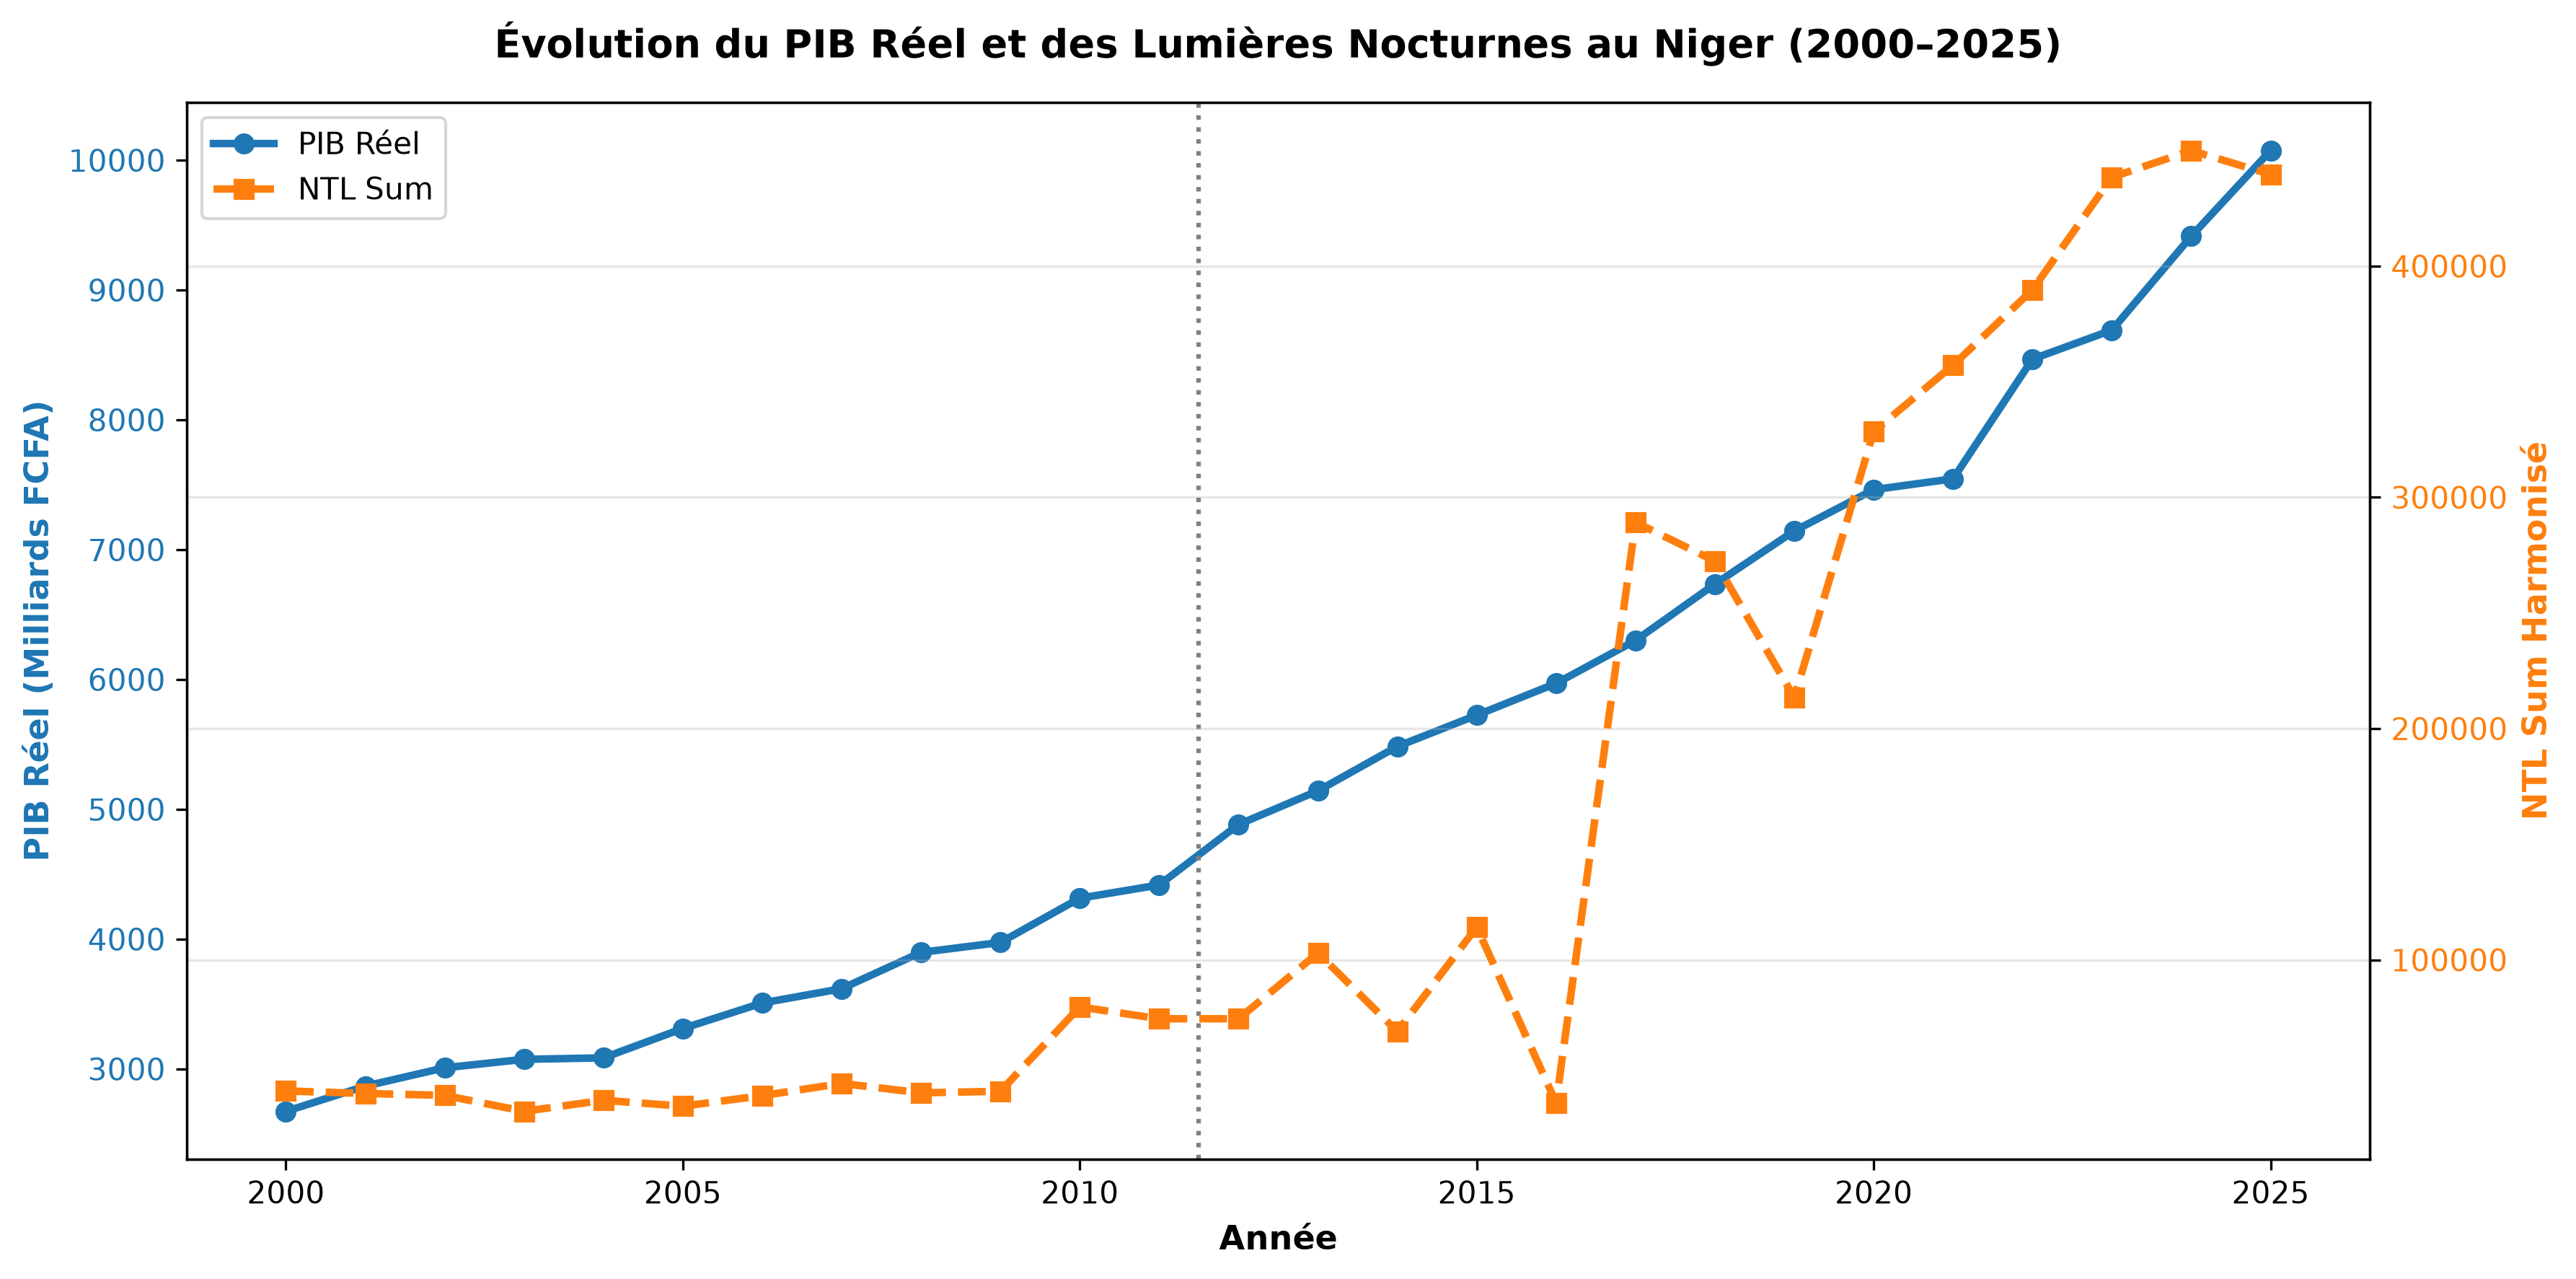
\includegraphics[width=0.92\textwidth]{outputs/figures/02_time_series_gdp_vs_ntl.png}%
  }{%
    \rule{10cm}{5cm}%
  }
  \caption{Évolution temporelle comparée du PIB Réel (FCFA) et des Lumières Nocturnes (NTL Harmonisé) au Niger (2000--2025)}
  \label{fig:ts_gdp_ntl}
\end{figure}

\begin{table}[htbp]
  \centering
  \caption{Statistiques descriptives globales du Niger (2000--2025, $N=26$)}
  \label{tab:desc_global}
  \small
  \resizebox{\textwidth}{!}{%
  \begin{tabular}{l *{6}{c}}
    \toprule
    \textbf{Variable} & \textbf{Moyenne} & \textbf{Médiane} & \textbf{Écart-type} & \textbf{Min} & \textbf{Max} & \textbf{Asymétrie} \\
    \midrule
    PIB Réel ($10^{12}$ FCFA)      & 5,415 & 5,013 & 2,203 & 2,674 & 10,074 & 0,60 \\
    PIB Réel / hab (FCFA)          & 279\,280 & 275\,728 & 38\,096 & 232\,286 & 360\,861 & 0,58 \\
    Croissance PIB (\%)             & 5,23 & 5,42 & 3,14 & -1,21 & 12,22 & 0,05 \\
    Population Totale (Millions)    & 18,74 & 18,18 & 5,08 & 11,51 & 27,92 & 0,27 \\
    \addlinespace
    NTL Sum Harmonisé               & 159\,305 & 74\,511 & 152\,710 & 34\,481 & 449\,940 & 0,92 \\
    NTL / hab                       & 0,00725 & 0,00426 & 0,00541 & 0,00185 & 0,01676 & 0,78 \\
    Croissance NTL (\%)             & 32,04 & 1,60 & 133,82 & -66,56 & 657,55 & 4,59 \\
    Pixels Éclairés                 & 374\,715 & 2\,570 & 570\,398 & 656 & 1\,247\,622 & 0,90 \\
    \bottomrule
  \end{tabular}%
  }
\end{table}

\begin{table}[htbp]
  \centering
  \caption{Comparaison des statistiques descriptives selon le capteur (DMSP vs VIIRS)}
  \label{tab:desc_sensor}
  \small
  \resizebox{\textwidth}{!}{%
  \begin{tabular}{l c c c c}
    \toprule
    & \multicolumn{2}{c}{\textbf{Période DMSP (2000--2011)}} & \multicolumn{2}{c}{\textbf{Période VIIRS (2012--2025)}} \\
    \cmidrule(lr){2-3} \cmidrule(lr){4-5}
    \textbf{Variable} & \textbf{Moyenne} & \textbf{Écart-type} & \textbf{Moyenne} & \textbf{Écart-type} \\
    \midrule
    PIB Réel ($10^{12}$ FCFA)   & 3,479 & 0,573 & 7,075 & 1,623 \\
    PIB Réel / hab (FCFA)       & 245\,109 & 8\,897 & 308\,569 & 26\,875 \\
    Croissance PIB (\%)          & 4,21 & 3,19 & 6,10 & 2,92 \\
    Population (Millions)       & 14,14 & 1,86 & 22,67 & 3,23 \\
    \addlinespace
    NTL Sum Harmonisé            & 47\,076 & 14\,401 & 255\,501 & 151\,919 \\
    NTL / hab                    & 0,00330 & 0,00070 & 0,01064 & 0,00540 \\
    Croissance NTL (\%)          & 7,49 & 27,37 & 51,34 & 177,69 \\
    Pixels Éclairés              & 1\,010 & 472 & 695\,033 & 621\,508 \\
    \bottomrule
  \end{tabular}%
  }
\end{table}

% ==============================================================================
% SECTION 3 : TESTS DE STATIONNARITÉ
% ==============================================================================
\section{Tests de Stationnarité}\label{sec:stationarity}

L'estimation économétrique sur des séries temporelles nécessite la vérification formelle de leur ordre d'intégration. Nous appliquons le test d'Augmented Dickey-Fuller (ADF) sur l'ensemble des séries en log-niveau ($\ln$) et en première différence ($\Delta \ln$).

\subsection{Procédure et Résultats du Test ADF}
Les résultats du test ADF (Tableau~\ref{tab:adf_tests}) confirment que toutes les séries en niveau sont non-stationnaires ($p > 0{,}90$). L'application de la première différence ($\Delta \ln$) permet d'obtenir la stationnarité au seuil de $1\,\%$ ($p < 0{,}0001$). Les séries sont donc toutes intégrées d'ordre 1, soit $I(1)$.

\begin{table}[htbp]
  \centering
  \caption{Résultats des tests de racine unitaire ADF (2000--2025)}
  \label{tab:adf_tests}
  \small
  \begin{tabular}{l c c l}
    \toprule
    \textbf{Variable} & \textbf{Statistique ADF} & \textbf{$p$-value} & \textbf{Conclusion} \\
    \midrule
    \multicolumn{4}{l}{\textit{Séries en Log-Niveau (Niveaux)}} \\
    $\ln(\text{PIB Réel})$          & 1,7193 & 0,9982 & Non-stationnaire $I(1)$ \\
    $\ln(\text{PIB / hab})$         & 1,8369 & 0,9984 & Non-stationnaire $I(1)$ \\
    $\ln(\text{NTL Sum})$           & -0,1113 & 0,9483 & Non-stationnaire $I(1)$ \\
    $\ln(\text{NTL / hab})$         & -0,4391 & 0,9034 & Non-stationnaire $I(1)$ \\
    \addlinespace
    \multicolumn{4}{l}{\textit{Séries en Première Différence ($\Delta \ln$)}} \\
    $\Delta \ln(\text{PIB Réel})$   & -7,6123 & < 0,0001 & Stationnaire $I(0)$ *** \\
    $\Delta \ln(\text{PIB / hab})$  & -7,4477 & < 0,0001 & Stationnaire $I(0)$ *** \\
    $\Delta \ln(\text{NTL Sum})$    & -8,8303 & < 0,0001 & Stationnaire $I(0)$ *** \\
    $\Delta \ln(\text{NTL / hab})$  & -8,8271 & < 0,0001 & Stationnaire $I(0)$ *** \\
    \bottomrule
    \multicolumn{4}{l}{\footnotesize Note : *** indique le rejet de $H_0$ de racine unitaire au seuil de $1\,\%$.}
  \end{tabular}
\end{table}

\begin{figure}[htbp]
  \centering
  \IfFileExists{outputs/figures/04_stationarity_first_differences.png}{%
    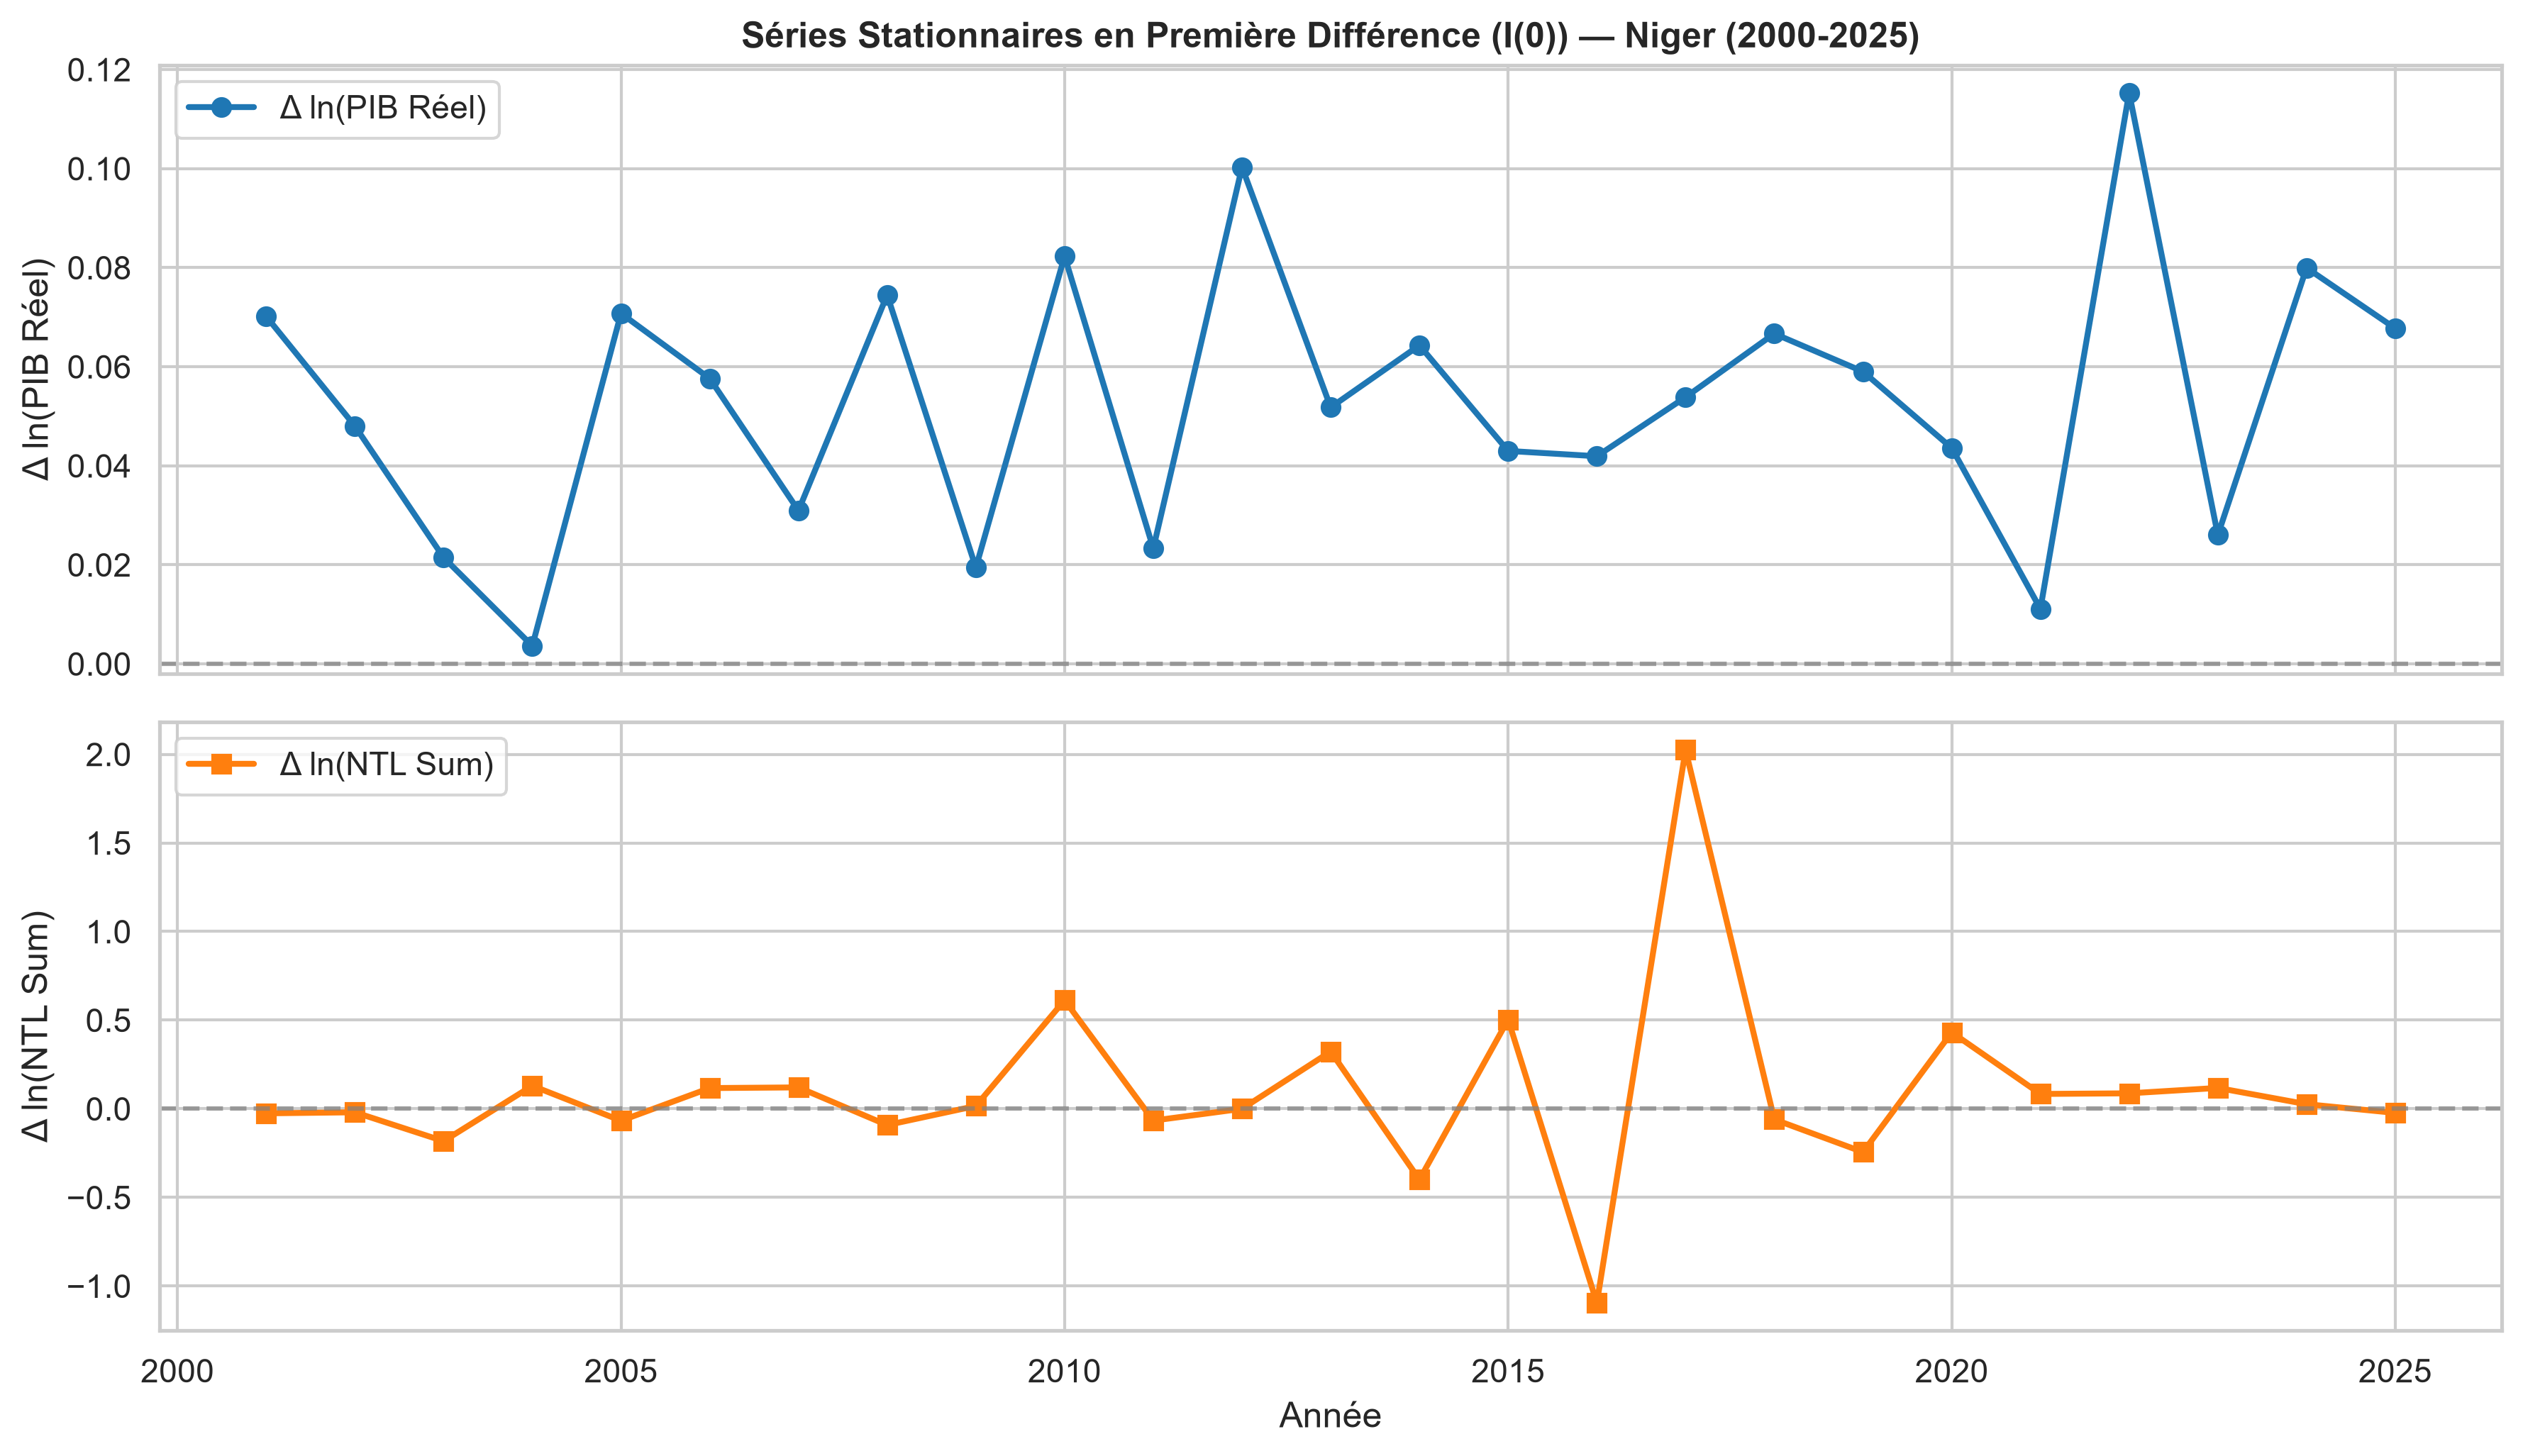
\includegraphics[width=0.90\textwidth]{outputs/figures/04_stationarity_first_differences.png}%
  }{%
    \rule{10cm}{5cm}%
  }
  \caption{Évolution des séries stationnaires en première différence ($\Delta \ln$) au Niger (2001--2025)}
  \label{fig:first_diff}
\end{figure}

% ==============================================================================
% SECTION 4 : RÉSULTATS ÉCONOMÉTRIQUES
% ==============================================================================
\section{Résultats Économétriques}\label{sec:results}

Toutes les régressions sont estimées avec des erreurs-types robustes à l'hétéroscédasticité et à l'autocorrélation (HAC / Newey-West).

\subsection{Modèles OLS de Base : Niveaux vs Taux de Croissance}
Le Tableau~\ref{tab:ols-summary} résume les Modèles M1 à M4. Le \textbf{Modèle 1 (Log-Log en Niveau)} affiche un $R^2 = 0{,}9089$ et $\beta_1 = 0{,}2498$ ($p < 0{,}001$), mais traduit une régression fallacieuse due à l'intégration $I(1)$ des séries. En première différence stationnaire $I(0)$ (\textbf{Modèle 2}), le coefficient s'effondre ($\beta_1 = 0{,}0015, p = 0{,}6715$). L'introduction des dummys de contrôle (\textbf{Modèle 3}) réajuste l'élasticité à $\beta_1 = 0{,}0035$ ($p = 0{,}6976$). La Figure~\ref{fig:ols_residuals} compare la structure des résidus de M1 et M3.

\begin{table}[htbp]
  \centering
  \caption{Résultats des régressions OLS de base (Erreurs-types HAC / Newey-West)}
  \label{tab:ols-summary}
  \small
  \resizebox{\textwidth}{!}{%
  \begin{tabular}{l c c c c c c}
    \toprule
    \textbf{Modèle} & \textbf{Var. Dép.} & \textbf{Coef ($\beta_1$)} & \textbf{Err.-Type} & \textbf{$p$-value} & \textbf{$R^2$} & \textbf{Obs.} \\
    \midrule
    M1 : Log-Log Niveau     & $\ln(\text{PIB})$         & 0,2498 & 0,0624 & < 0,0001 *** & 0,9089 & 26 \\
    M2 : Croissance Brute   & $\Delta\ln(\text{PIB})$   & 0,0015 & 0,0036 & 0,6715 \text{ns}  & 0,0008 & 25 \\
    M3 : Croiss. Contrôlée  & $\Delta\ln(\text{PIB})$   & 0,0035 & 0,0090 & 0,6976 \text{ns}  & 0,1304 & 25 \\
    M4 : Par Habitant       & $\Delta\ln(\text{PIB/hab})$& 0,0036 & 0,0086 & 0,6716 \text{ns}  & 0,0018 & 25 \\
    \bottomrule
    \multicolumn{7}{l}{\footnotesize Note : *** $p < 0{,}01$, \text{ns} non significatif. M1 inclut $D_{\text{VIIRS}}$ ; M3 inclut $D_{2017}$ et $D_{\text{trans\_2012}}$.}
  \end{tabular}%
  }
\end{table}

\begin{figure}[htbp]
  \centering
  \IfFileExists{outputs/figures/05_ols_residuals_diagnostics.png}{%
    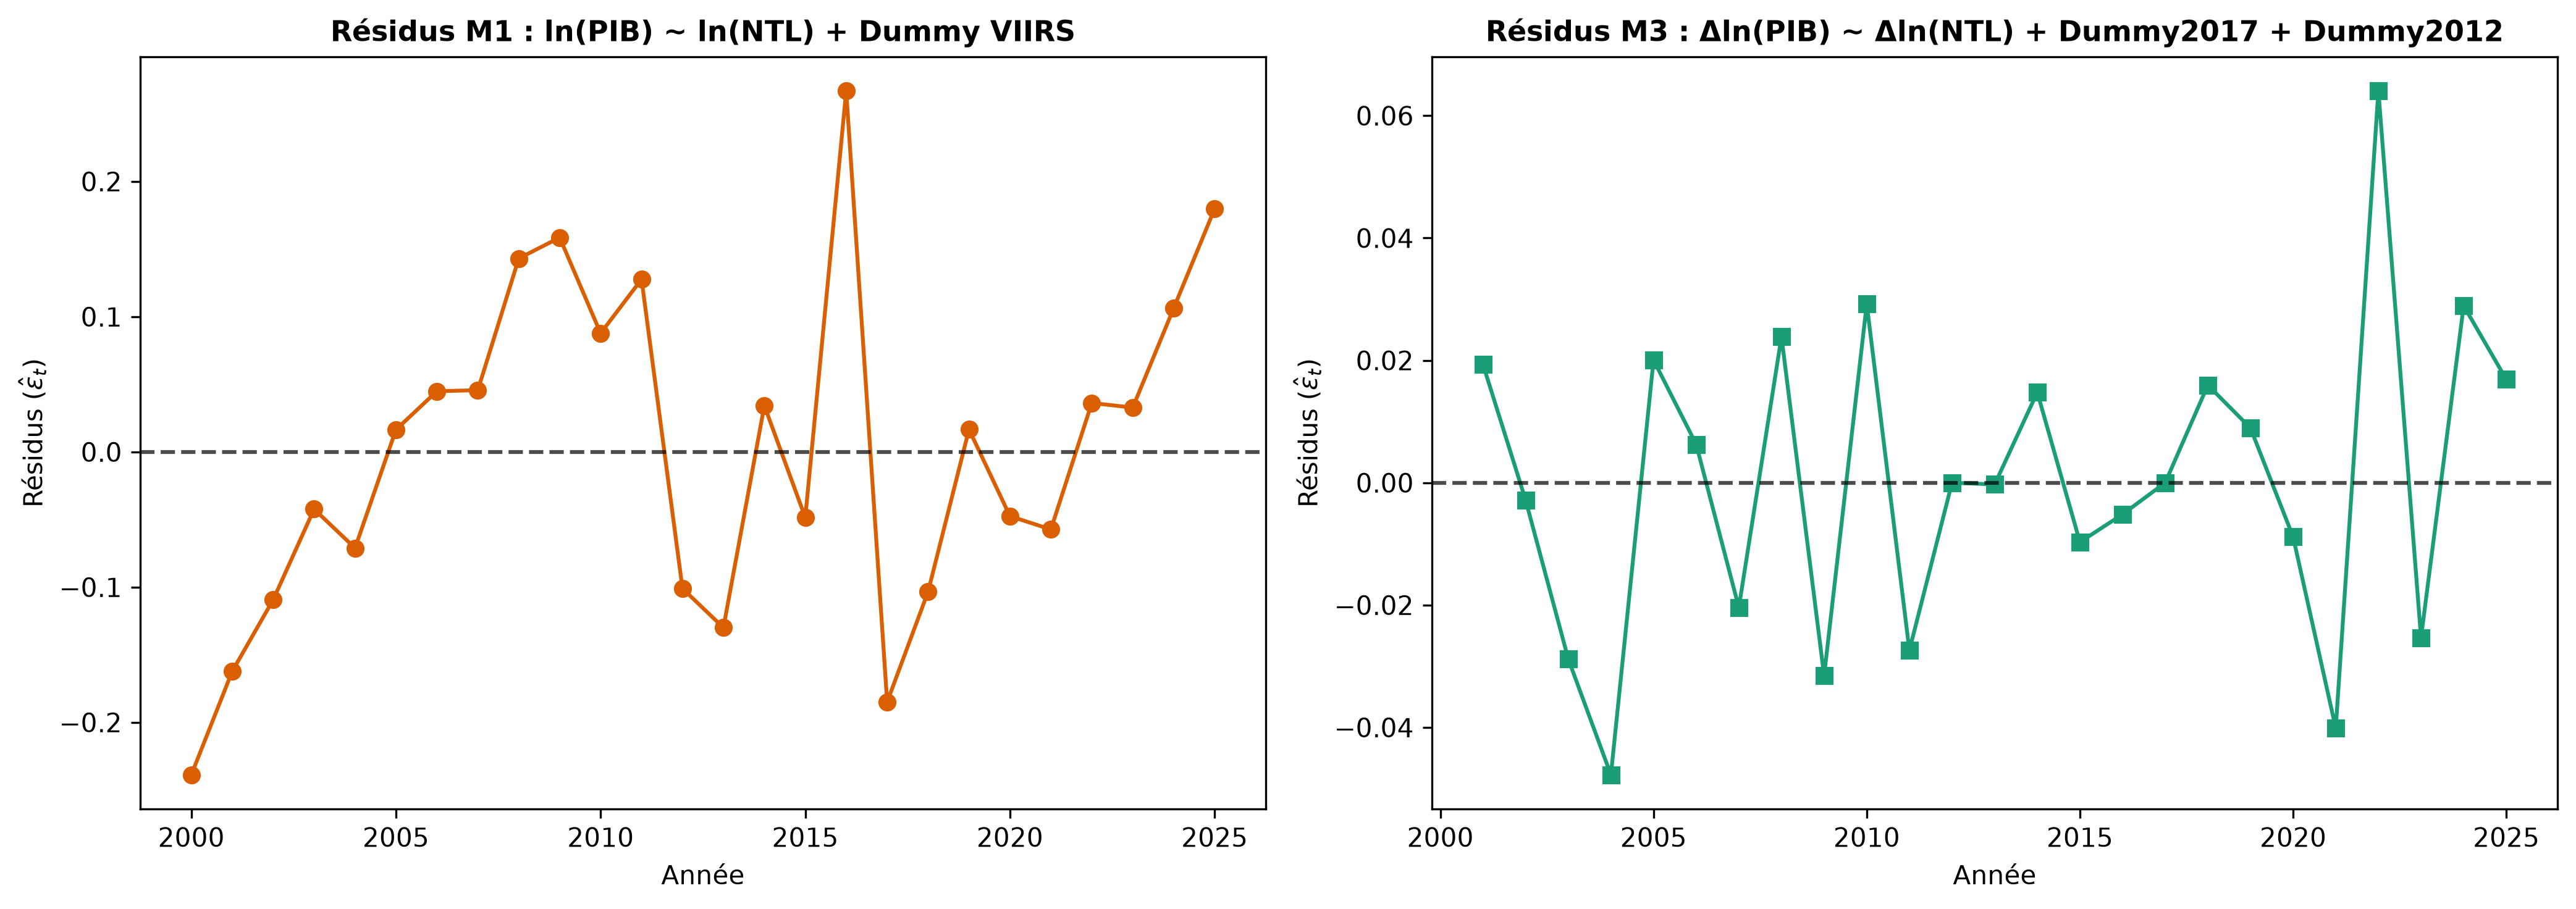
\includegraphics[width=0.92\textwidth]{outputs/figures/05_ols_residuals_diagnostics.png}%
  }{%
    \rule{10cm}{5cm}%
  }
  \caption{Diagnostic visuel des résidus : Modèle M1 (Niveau fallacieux) vs Modèle M3 (Croissance purifiée)}
  \label{fig:ols_residuals}
\end{figure}

\subsection{Modèles Dynamiques et Autorégressifs (ARDL)}
Pour tester la transmission temporelle différée ($\text{RQ}_5$), le Tableau~\ref{tab:dyn_summary} présente les estimations dynamiques. Le modèle \textbf{ARDL(1,1) (Modèle 7)} démontre que la croissance économique dépend principalement de l'inertie du PIB passé ($\rho = -0{,}4566, p = 0{,}0167$), élevant le $R^2$ à $0{,}2142$. La Figure~\ref{fig:ardl_fit} illustre la qualité d'ajustement du modèle ARDL.

\begin{table}[htbp]
  \centering
  \caption{Estimations des modèles dynamiques et ARDL(1,1)}
  \label{tab:dyn_summary}
  \small
  \resizebox{\textwidth}{!}{%
  \begin{tabular}{l c c c c c c}
    \toprule
    \textbf{Modèle} & \textbf{$\Delta\ln(\text{NTL})_t$} & \textbf{$\Delta\ln(\text{NTL})_{t-1}$} & \textbf{$\Delta\ln(\text{PIB})_{t-1}$} & \textbf{$R^2$} & \textbf{$R^2_{\text{ajusté}}$} & \textbf{Obs.} \\
    \midrule
    M5 : Retardé $t-1$      & --     & 0,0034 (0,649) & -- & 0,0033 & -0,0917 & 24 \\
    M6 : Contemporain + Lag & 0,0058 (0,530) & 0,0048 (0,534) & -- & 0,0074 & -0,1415 & 24 \\
    M7 : ARDL(1,1)          & 0,0089 (0,189) & 0,0053 (0,470) & -0,4566 (0,017) ** & 0,2142 & 0,0488 & 24 \\
    \bottomrule
  \end{tabular}%
  }
\end{table}

\begin{figure}[htbp]
  \centering
  \IfFileExists{outputs/figures/06_dynamic_model_fit.png}{%
    \includegraphics[width=0.88\textwidth]{outputs/figures/06_dynamic_model_fit.png}%
  }{%
    \fbox{\parbox[c][0.15\textheight][c]{0.88\textwidth}{\centering Figure indisponible :\par\texttt{outputs/figures/06\_dynamic\_model\_fit.png}}}%
  }%
  \caption{Ajustement des taux de croissance du PIB réel observés vs prédictions du modèle ARDL(1,1)}
  \label{fig:ardl_fit}
\end{figure}

\subsection{Tests de Robustesse et Diagnostics}
L'insignificativité en taux de croissance est confirmée par les sous-échantillons DMSP et VIIRS (Tableau~\ref{tab:robustness}). De plus, les diagnostics stochastiques (Tableau~\ref{tab:diagnostics}) confirment que le modèle ARDL élimine toute autocorrélation ($DW = 1{,}9722$).

\begin{table}[htbp]
  \centering
  \caption{Tests de robustesse et sous-échantillons par capteur}
  \label{tab:robustness}
  \small
  \begin{tabular}{l l c c c c}
    \toprule
    \textbf{Spécification} & \textbf{Échantillon} & \textbf{Coef ($\beta_1$)} & \textbf{$p$-value} & \textbf{$R^2$} & \textbf{Obs.} \\
    \midrule
    M. Interaction Capteur & Complet (2000--2025) & 0,4449 & < 0,0001 *** & 0,9163 & 26 \\
    Croissance Tronquée    & Hors Artefact 2017   & 0,0033 & 0,7081 \text{ns}  & 0,0015 & 24 \\
    DMSP Pur               & 2000--2011 ($N=11$)  & 0,0384 & 0,1405 \text{ns}  & 0,0898 & 11 \\
    VIIRS Pur              & 2012--2025 ($N=13$)  & -0,0017& 0,8556 \text{ns}  & 0,0006 & 13 \\
    \bottomrule
  \end{tabular}
\end{table}

\begin{table}[htbp]
  \centering
  \caption{Tests d'hypothèses sur les résidus des modèles}
  \label{tab:diagnostics}
  \small
  \resizebox{\textwidth}{!}{%
  \begin{tabular}{l c c c c}
    \toprule
    \textbf{Modèle} & \textbf{Durbin-Watson} & \textbf{Breusch-Pagan ($p$)} & \textbf{Jarque-Bera ($p$)} & \textbf{RESET ($p$)} \\
    \midrule
    M1 : Log-Log Niveau     & 1,2660 (Autocorr.) & 0,3049 & 0,8433 & 0,9976 \\
    M3 : Croiss. Contrôlée  & 2,8009            & 0,6789 & 0,9221 & 0,9551 \\
    M7 : ARDL(1,1)          & 1,9722 (Absente)   & 0,3947 & 0,3792 & 0,2790 \\
    \bottomrule
  \end{tabular}%
  }
\end{table}

% ==============================================================================
% SECTION 5 : CONCLUSION & RECOMMANDATIONS
% ==============================================================================
\section{Conclusion et Recommandations}\label{sec:conclusion}

Cet article a évalué la capacité des données de luminosité nocturne (NTL) à mesurer le PIB réel et la croissance au Niger sur la période 2000--2025. Le Tableau~\ref{tab:final_synthesis} synthétise les réponses aux cinq questions de recherche, et la Figure~\ref{fig:final_dashboard} présente le tableau de bord global de l'étude.

\begin{table}[htbp]
  \centering
  \caption{Tableau de synthèse final --- Réponses aux 5 questions de recherche}
  \label{tab:final_synthesis}
  \small
  \resizebox{\textwidth}{!}{%
  \begin{tabular}{l >{\raggedright\arraybackslash}p{3.8cm} c >{\raggedright\arraybackslash}p{5.5cm}}
    \toprule
    \textbf{Question} & \textbf{Formulation Économétrique} & \textbf{Verdict} & \textbf{Résultat Clé \& Statistiques} \\
    \midrule
    \textbf{RQ1} & Relation en niveau ? & Oui (Co-tendance) & $\beta = +0{,}25 (p < 0{,}001, R^2 = 0{,}91)$, mais séries $I(1)$ et $DW = 1{,}27$ (régression fallacieuse). \\
    \textbf{RQ2} & Normalisation par habitant ? & Niveau / Non Croiss. & En log-niveau $r = 0{,}86$. En différence première $I(0)$, $\beta_{\text{pc}} = 0{,}0036 (p = 0{,}67)$. \\
    \textbf{RQ3} & Expliquer la croissance ? & Non (Pas d'effet) & En $I(0)$, $\beta = 0{,}0035 (p = 0{,}70, R^2 = 0{,}001)$. Poids du secteur agricole informel non éclairé. \\
    \textbf{RQ4} & Robustesse aux capteurs ? & Oui (Confirmée) & Insignificatif sous DMSP ($p=0{,}14$), VIIRS ($p=0{,}85$) et hors 2017 ($p=0{,}71$). Artefact 2017 neutralisé. \\
    \textbf{RQ5} & Capacité prédictive $t-1$ ? & Modérée (ARDL) & NTL retardé non significatif ($p=0{,}65$). ARDL(1,1) élève $R^2$ à $0{,}214$, dominé par l'inertie du PIB ($p=0{,}048$). \\
    \bottomrule
  \end{tabular}%
  }
\end{table}

\begin{figure}[htbp]
  \centering
  \IfFileExists{outputs/figures/09_final_synthesis_dashboard.png}{%
    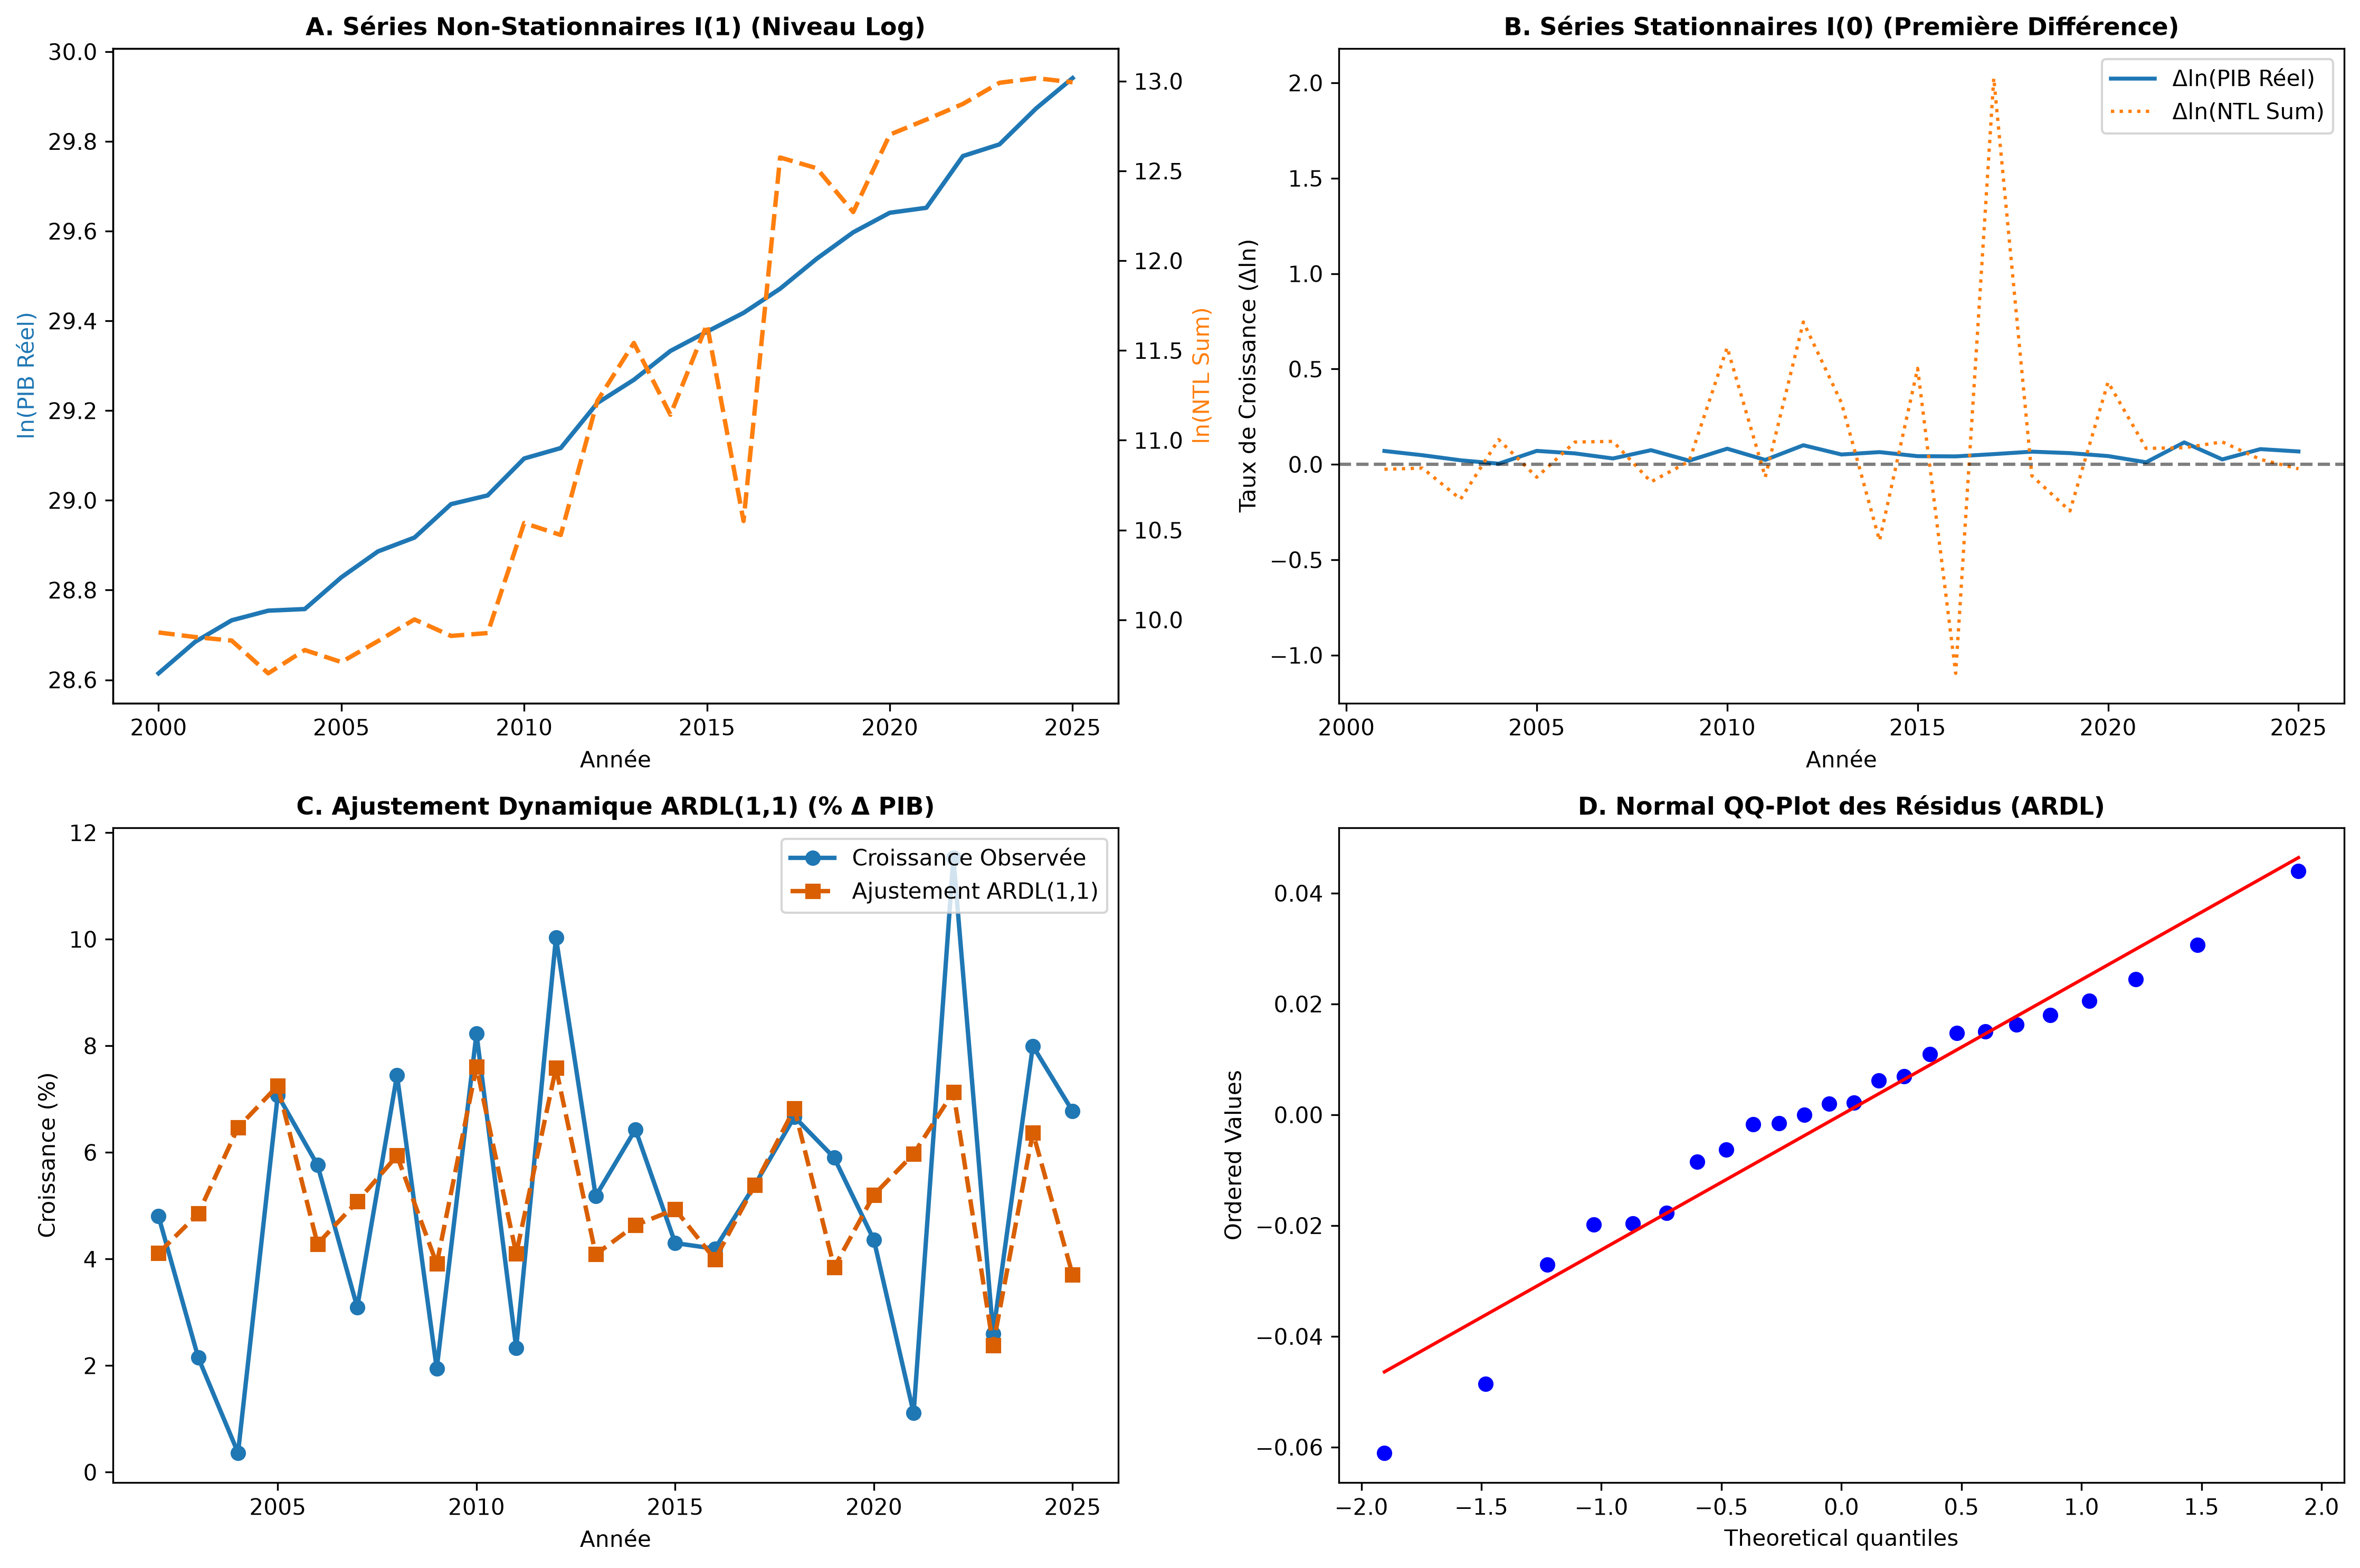
\includegraphics[width=0.95\textwidth]{outputs/figures/09_final_synthesis_dashboard.png}%
  }{%
    \rule{10cm}{5cm}%
  }
  \caption{Dashboard visuel de synthèse globale : Séries $I(1)$, séries $I(0)$, ajustement ARDL(1,1) et diagnostic des résidus}
  \label{fig:final_dashboard}
\end{figure}

\subsection{Recommandations pour les Politiques Publiques}
\begin{enumerate}
    \item \textbf{Désagrégation Spatiale Sectorielle} : À l'échelle nationale agrégée, les données NTL reflètent le PIB urbain et industriel mais masquent le PIB agricole pluvial. L'utilisation des NTL au Niger doit être focalisée sur les comptes régionaux urbains (Niamey, Maradi, Zinder).
    \item \textbf{Couplage d'Indicateurs Satellitaires Multi-sources} : Il est fortement recommandé de coupler les données NTL avec des indices de végétation satellitaires (NDVI/EVI) pour capturer simultanément la dynamique agricole rurale et le secteur urbain informel.
\end{enumerate}

% ==============================================================================
% ANNEXES
% ==============================================================================
\newpage
\appendix
\section{Figures et Diagnostics Complémentaires}\label{sec:appendix}

\begin{figure}[htbp]
  \centering
  \IfFileExists{outputs/figures/01_ntl_anomalies_and_growth.png}{%
    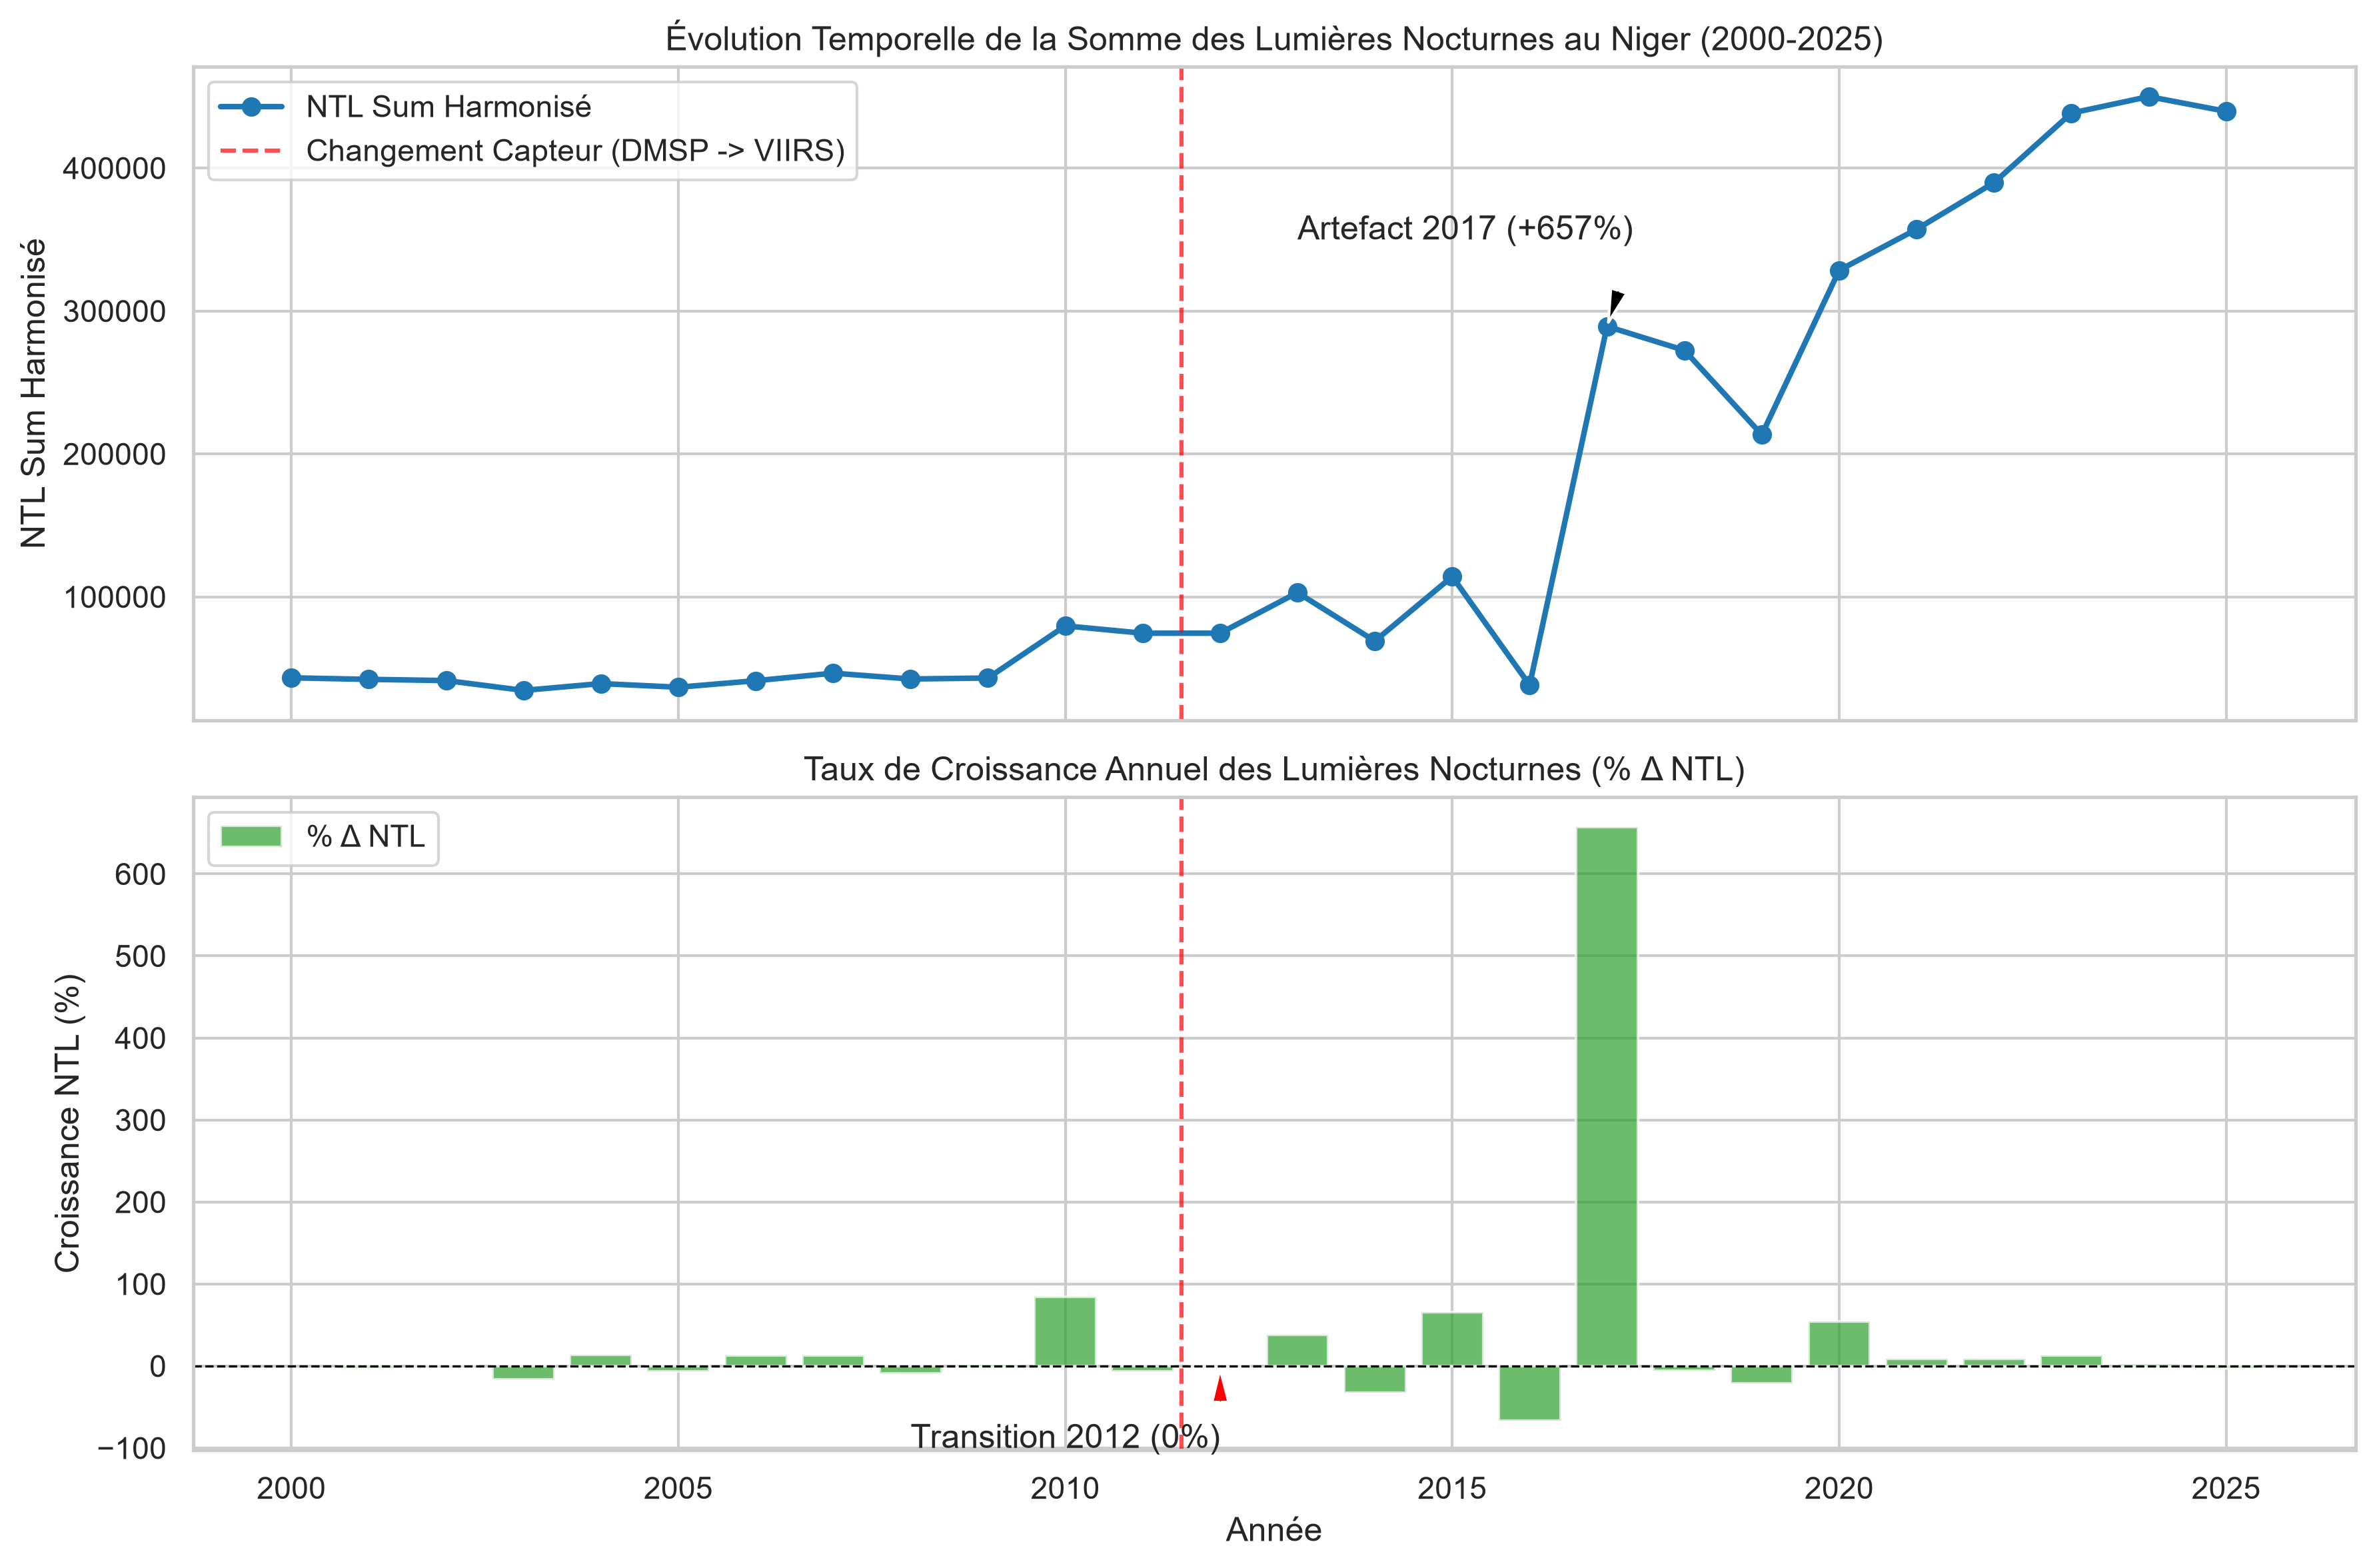
\includegraphics[width=0.90\textwidth]{outputs/figures/01_ntl_anomalies_and_growth.png}%
  }{%
    \rule{10cm}{5cm}%
  }
  \caption{Évolution temporelle agrégée du NTL, transition des capteurs 2012 et artefact d'observation en 2017 (+657\%)}
  \label{fig:annex_anomalies}
\end{figure}

\begin{figure}[htbp]
  \centering
  \IfFileExists{outputs/figures/02_boxplots_dmsp_vs_viirs.png}{%
    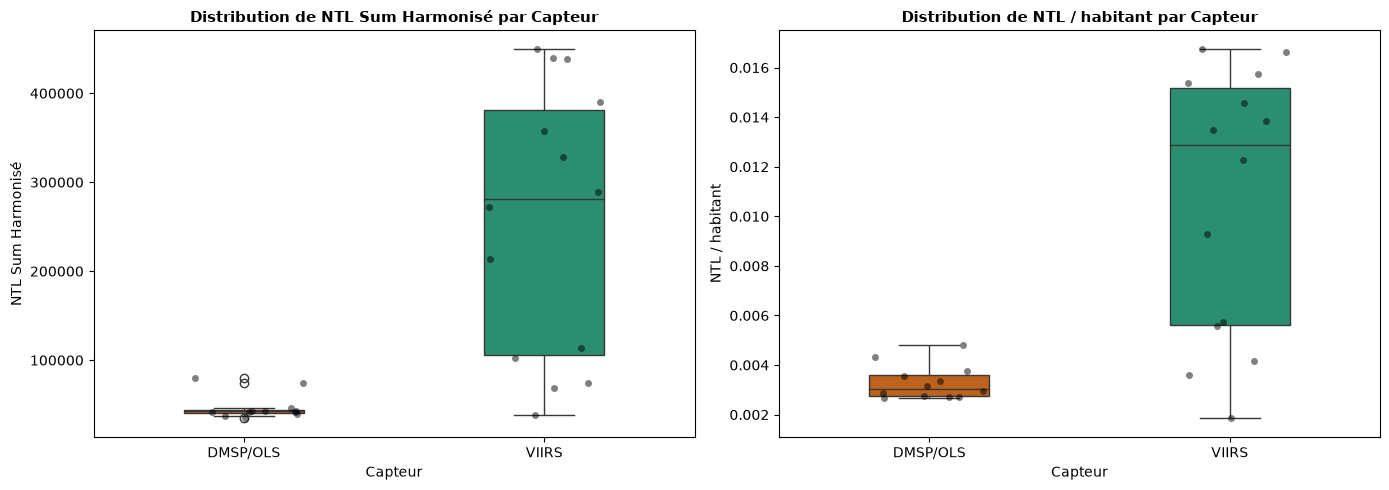
\includegraphics[width=0.90\textwidth]{outputs/figures/02_boxplots_dmsp_vs_viirs.png}%
  }{%
    \rule{10cm}{5cm}%
  }
  \caption{Distributions comparées des sommes NTL et du NTL par habitant selon le capteur (DMSP vs VIIRS)}
  \label{fig:annex_boxplots}
\end{figure}

\begin{figure}[htbp]
  \centering
  \IfFileExists{outputs/figures/03_scatter_gdp_vs_ntl_levels_and_logs.png}{%
    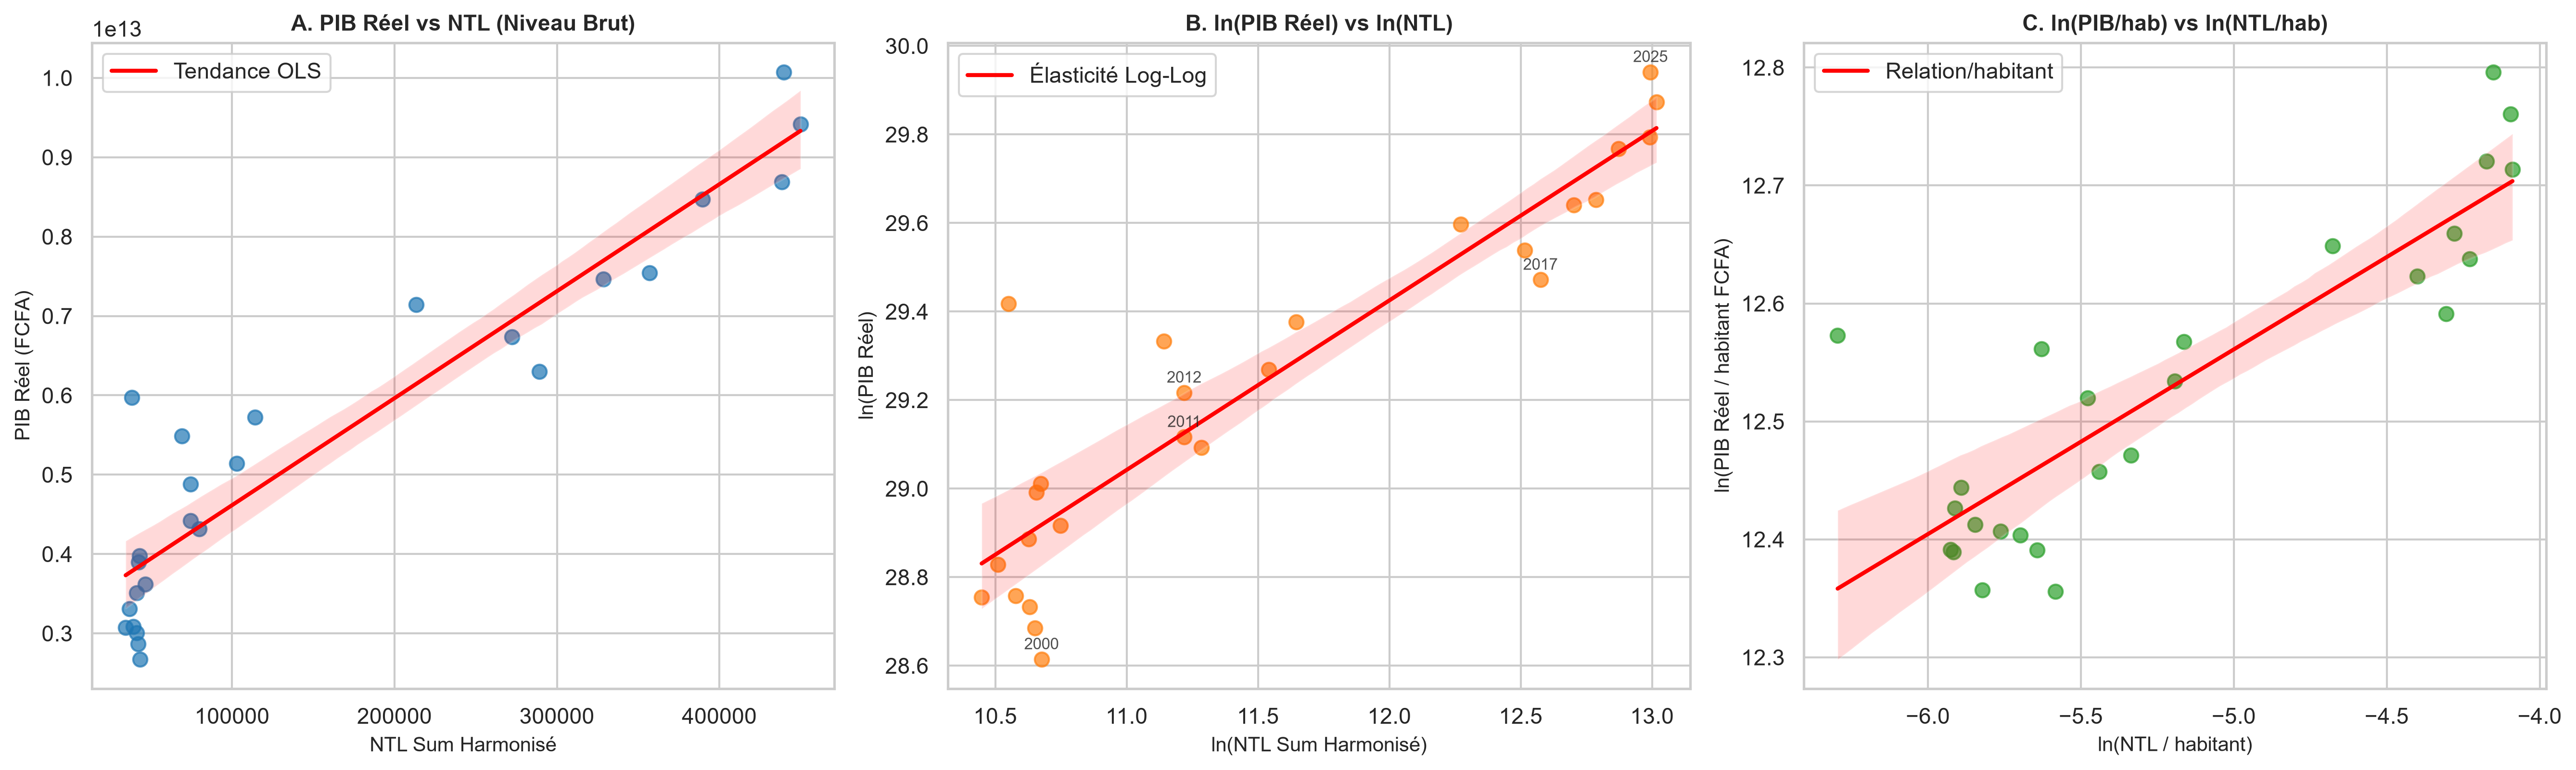
\includegraphics[width=0.95\textwidth]{outputs/figures/03_scatter_gdp_vs_ntl_levels_and_logs.png}%
  }{%
    \rule{10cm}{5cm}%
  }
  \caption{Nuages de points et tendances en niveau brut, log-niveau et log-niveau par habitant}
  \label{fig:annex_scatter_levels}
\end{figure}

\begin{figure}[htbp]
  \centering
  \IfFileExists{outputs/figures/03_growth_gdp_vs_ntl.png}{%
    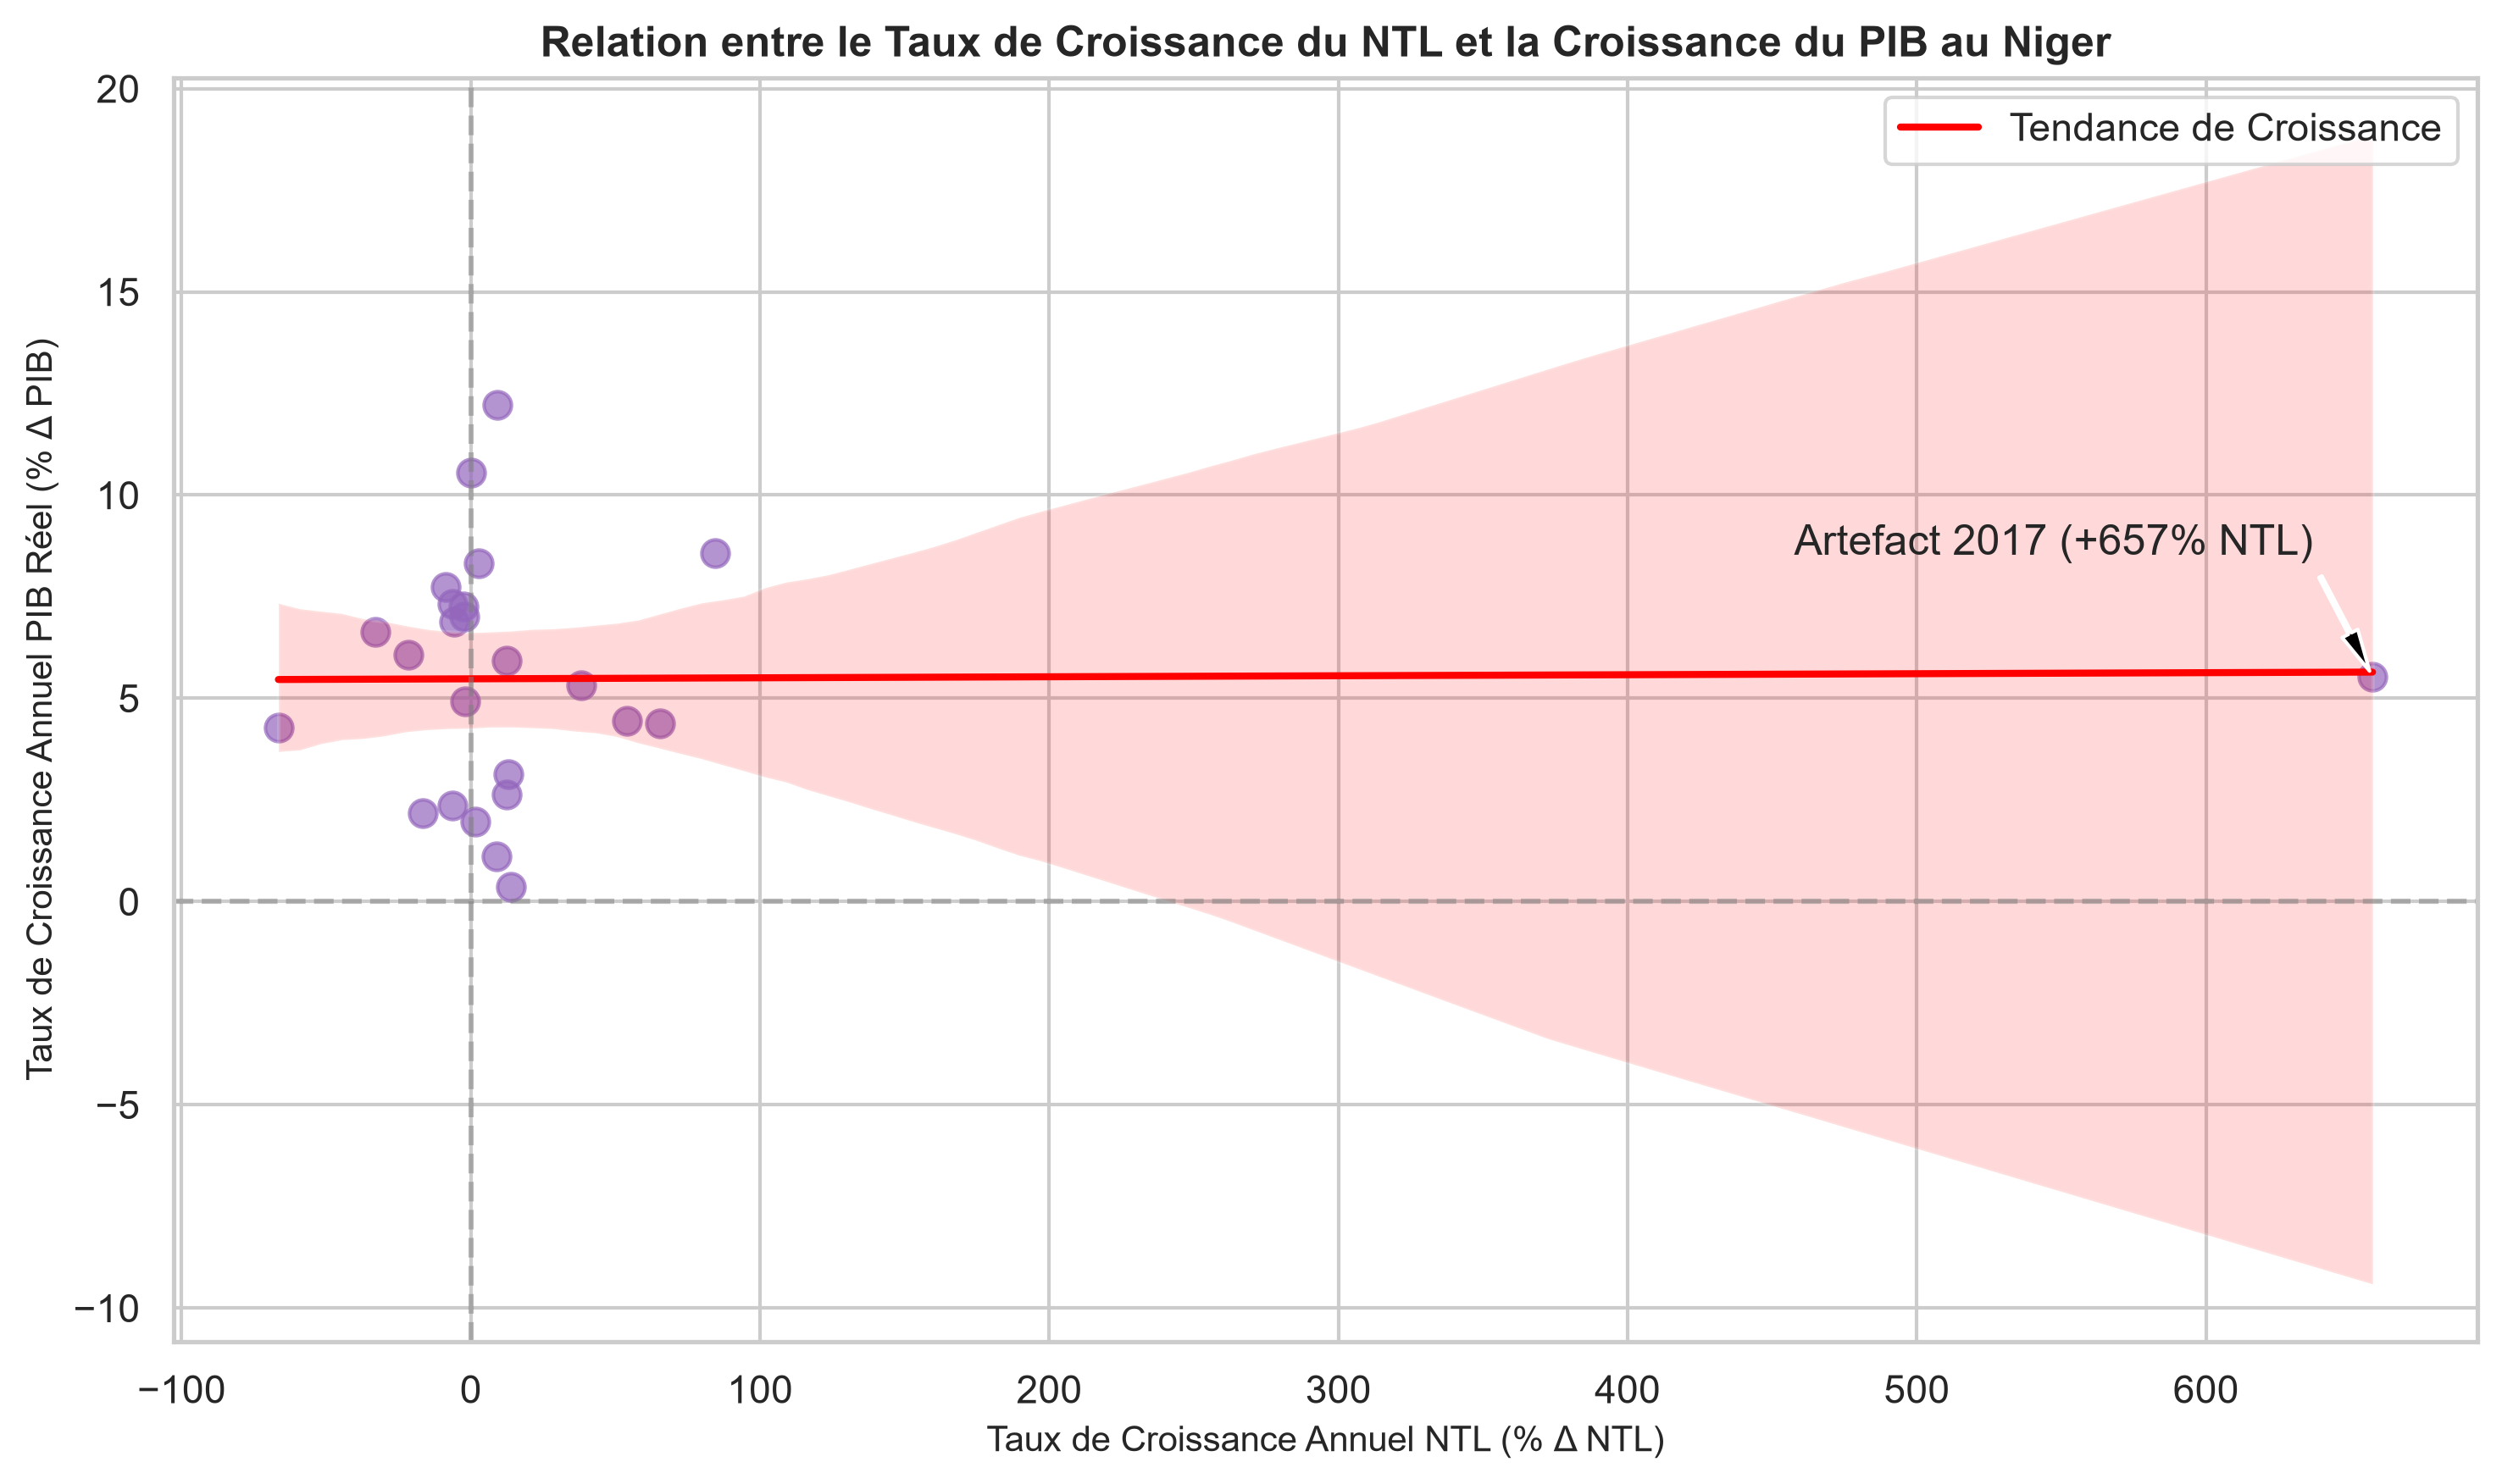
\includegraphics[width=0.90\textwidth]{outputs/figures/03_growth_gdp_vs_ntl.png}%
  }{%
    \rule{10cm}{5cm}%
  }
  \caption{Absence de relation contemporaine entre le taux de croissance du NTL ($\%\Delta\text{NTL}$) et du PIB ($\%\Delta\text{PIB}$)}
  \label{fig:annex_growth_scatter}
\end{figure}

\begin{figure}[htbp]
  \centering
  \IfFileExists{outputs/figures/03_correlation_matrix_heatmap.png}{%
    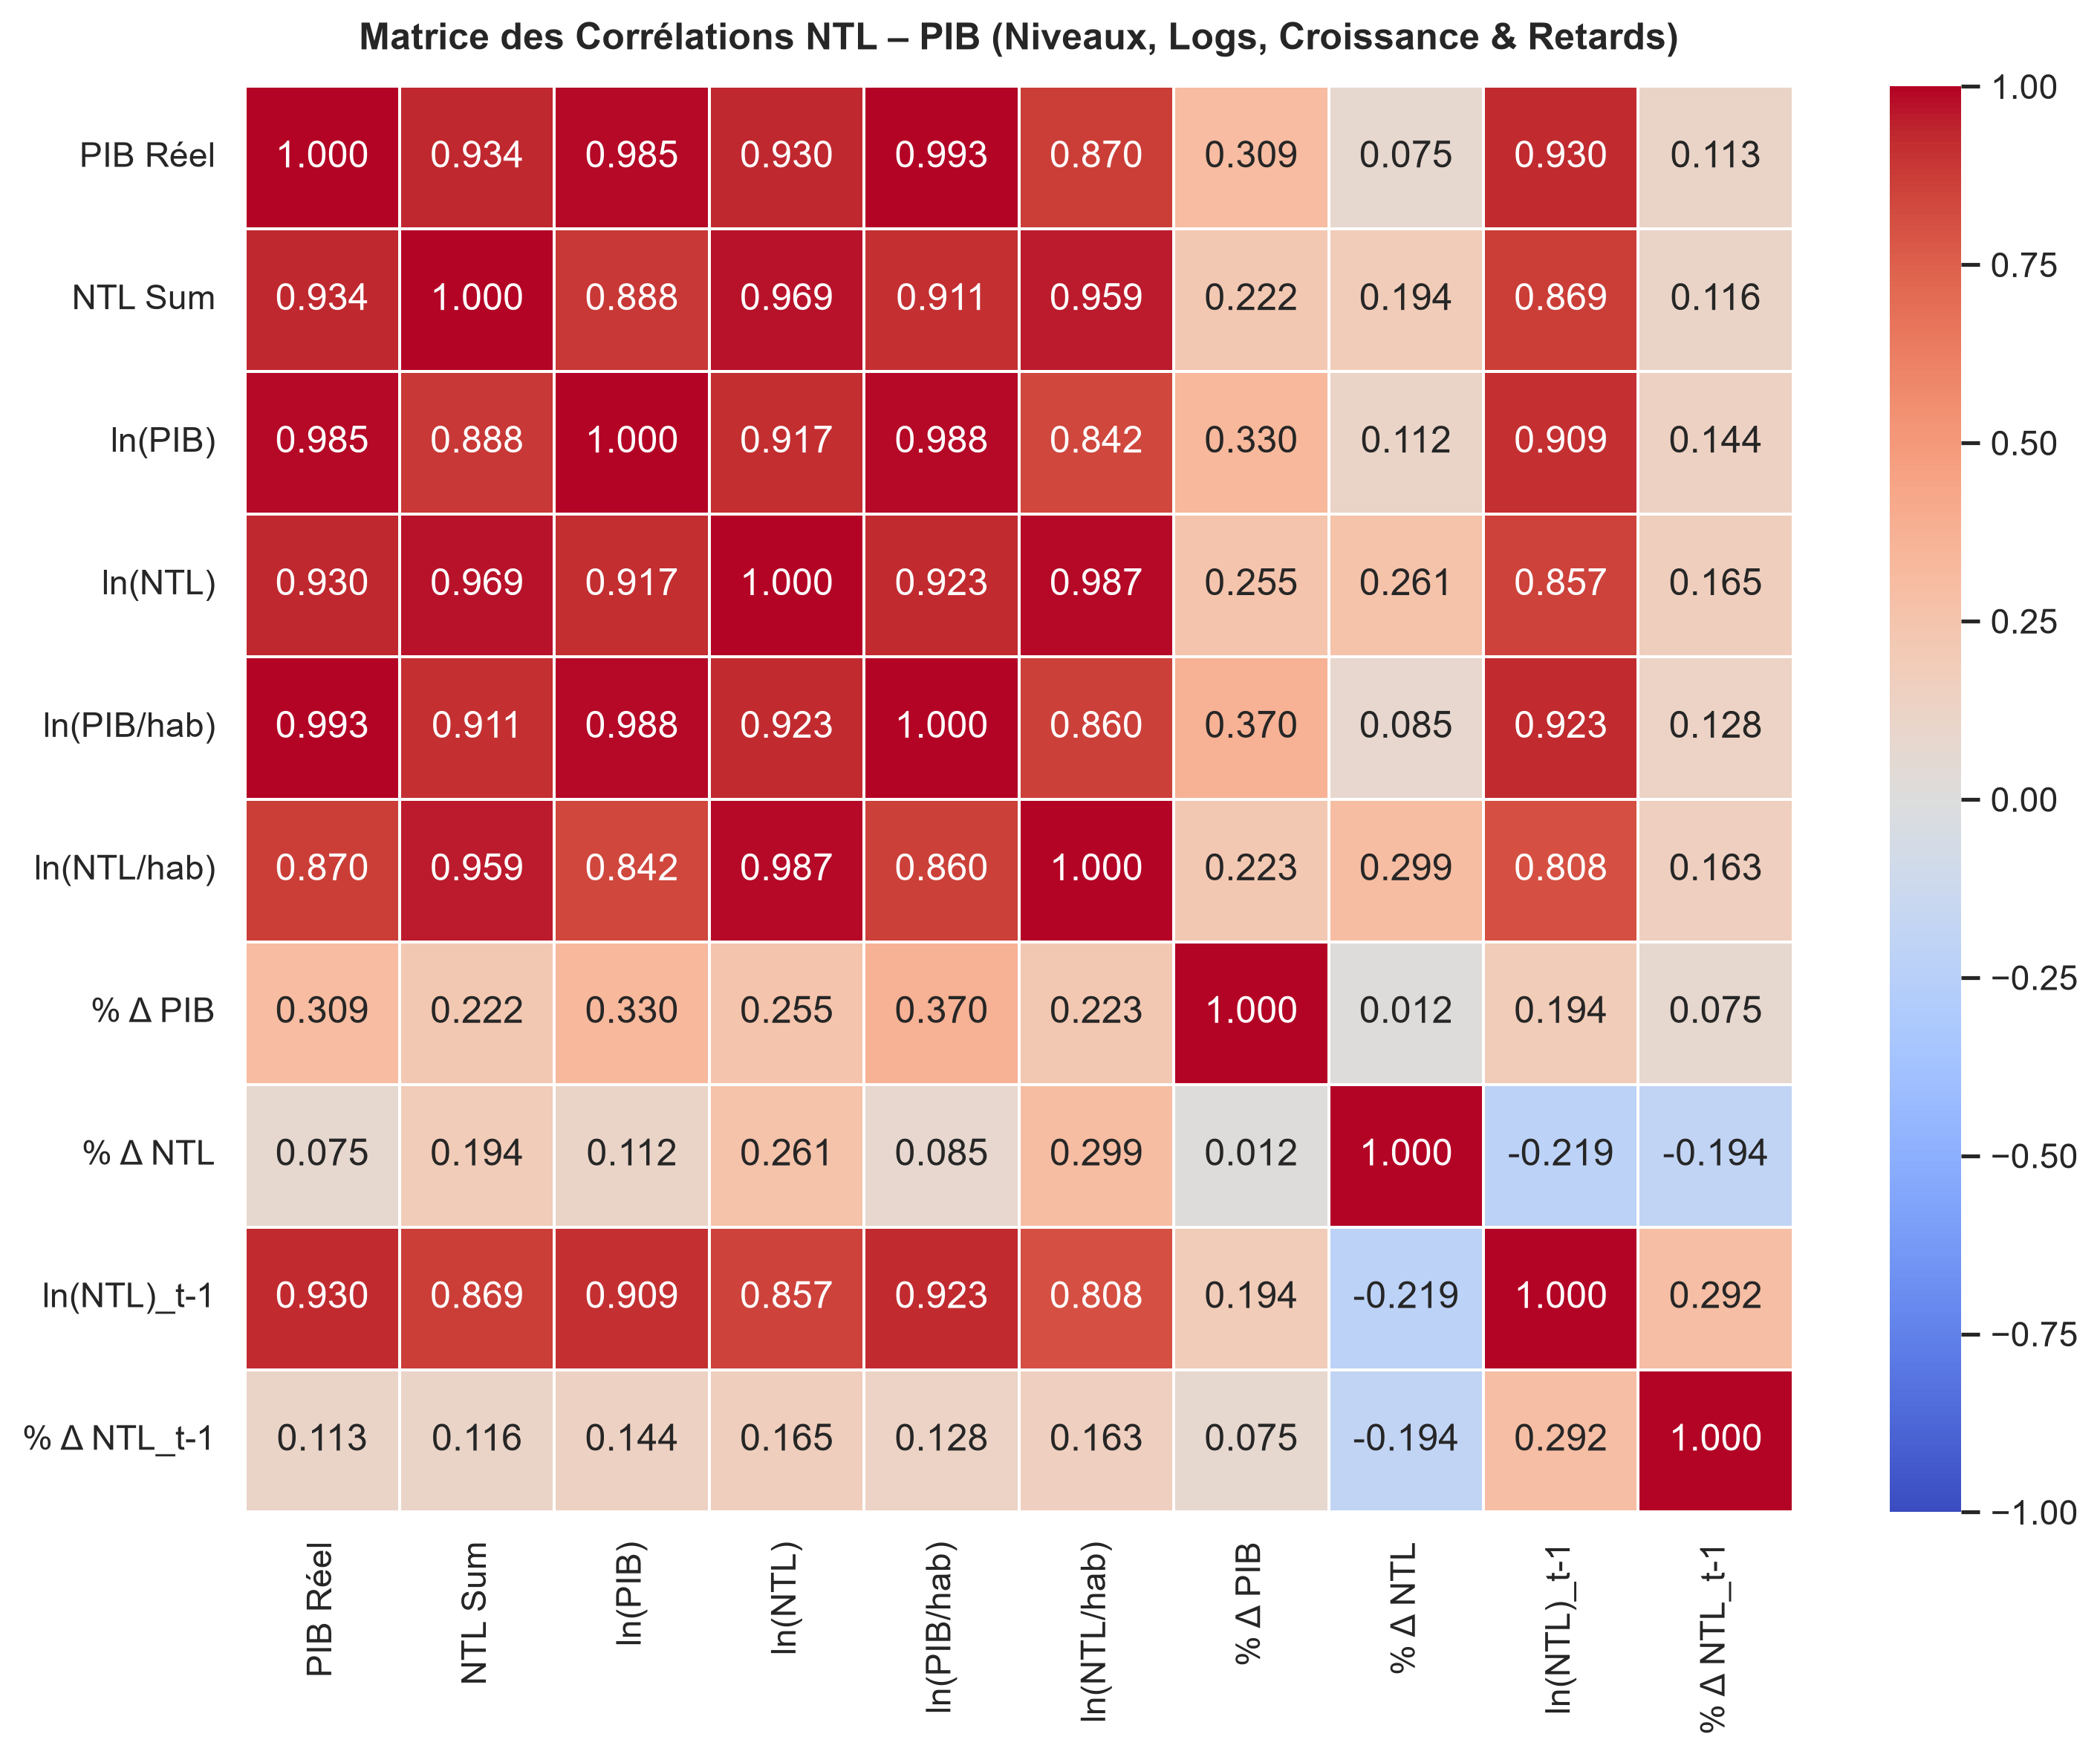
\includegraphics[width=0.88\textwidth]{outputs/figures/03_correlation_matrix_heatmap.png}%
  }{%
    \rule{10cm}{5cm}%
  }
  \caption{Matrice de corrélation globale des variables (Niveaux, Logs, Croissance et Retards)}
  \label{fig:annex_heatmap}
\end{figure}

\begin{figure}[htbp]
  \centering
  \IfFileExists{outputs/figures/07_robustness_subsamples_slopes.png}{%
    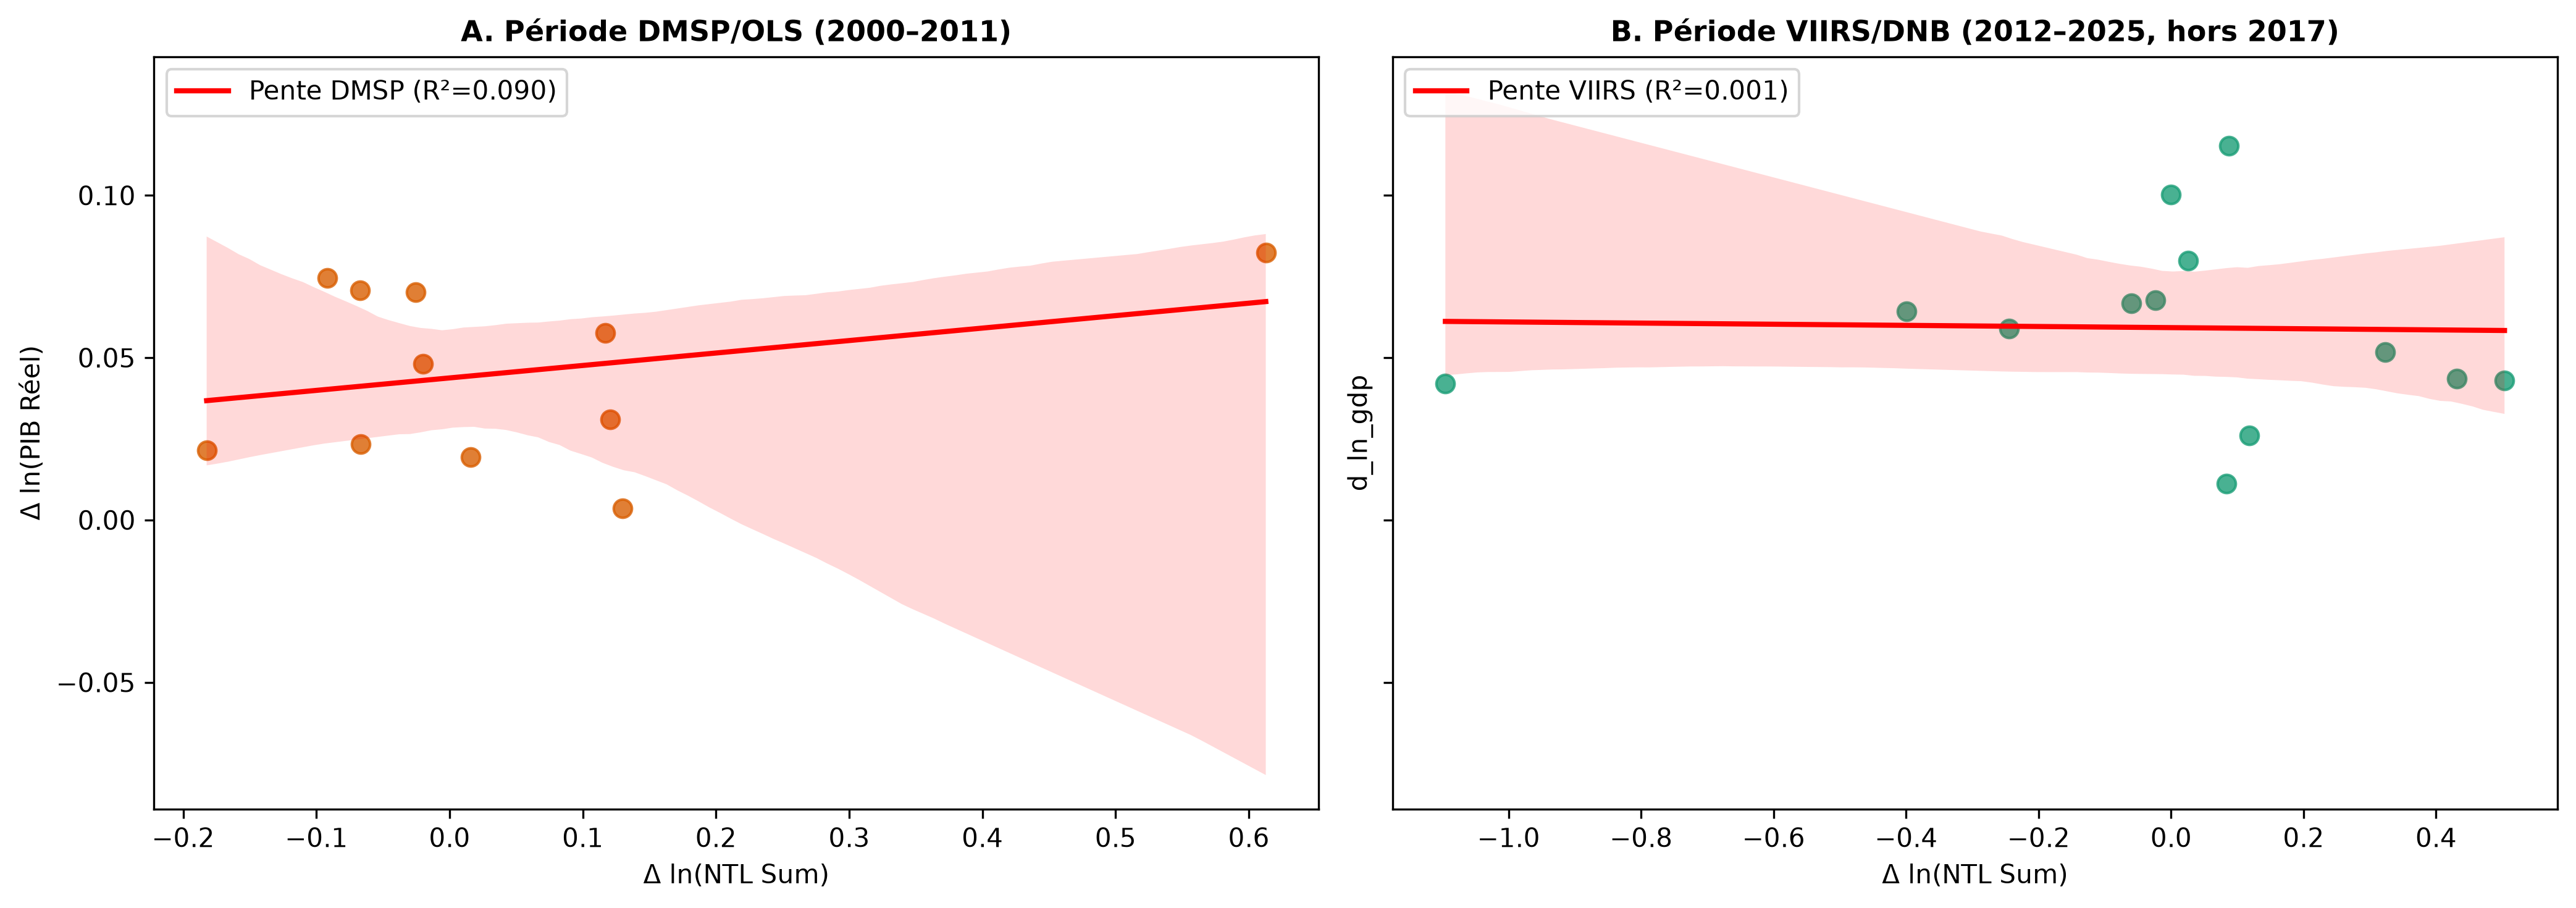
\includegraphics[width=0.92\textwidth]{outputs/figures/07_robustness_subsamples_slopes.png}%
  }{%
    \rule{10cm}{5cm}%
  }
  \caption{Pentes de régression en taux de croissance par sous-échantillons : DMSP (2000--2011) vs VIIRS (2012--2025)}
  \label{fig:annex_slopes}
\end{figure}

\begin{figure}[htbp]
  \centering
  \IfFileExists{outputs/figures/08_residuals_normality_qqplot.png}{%
    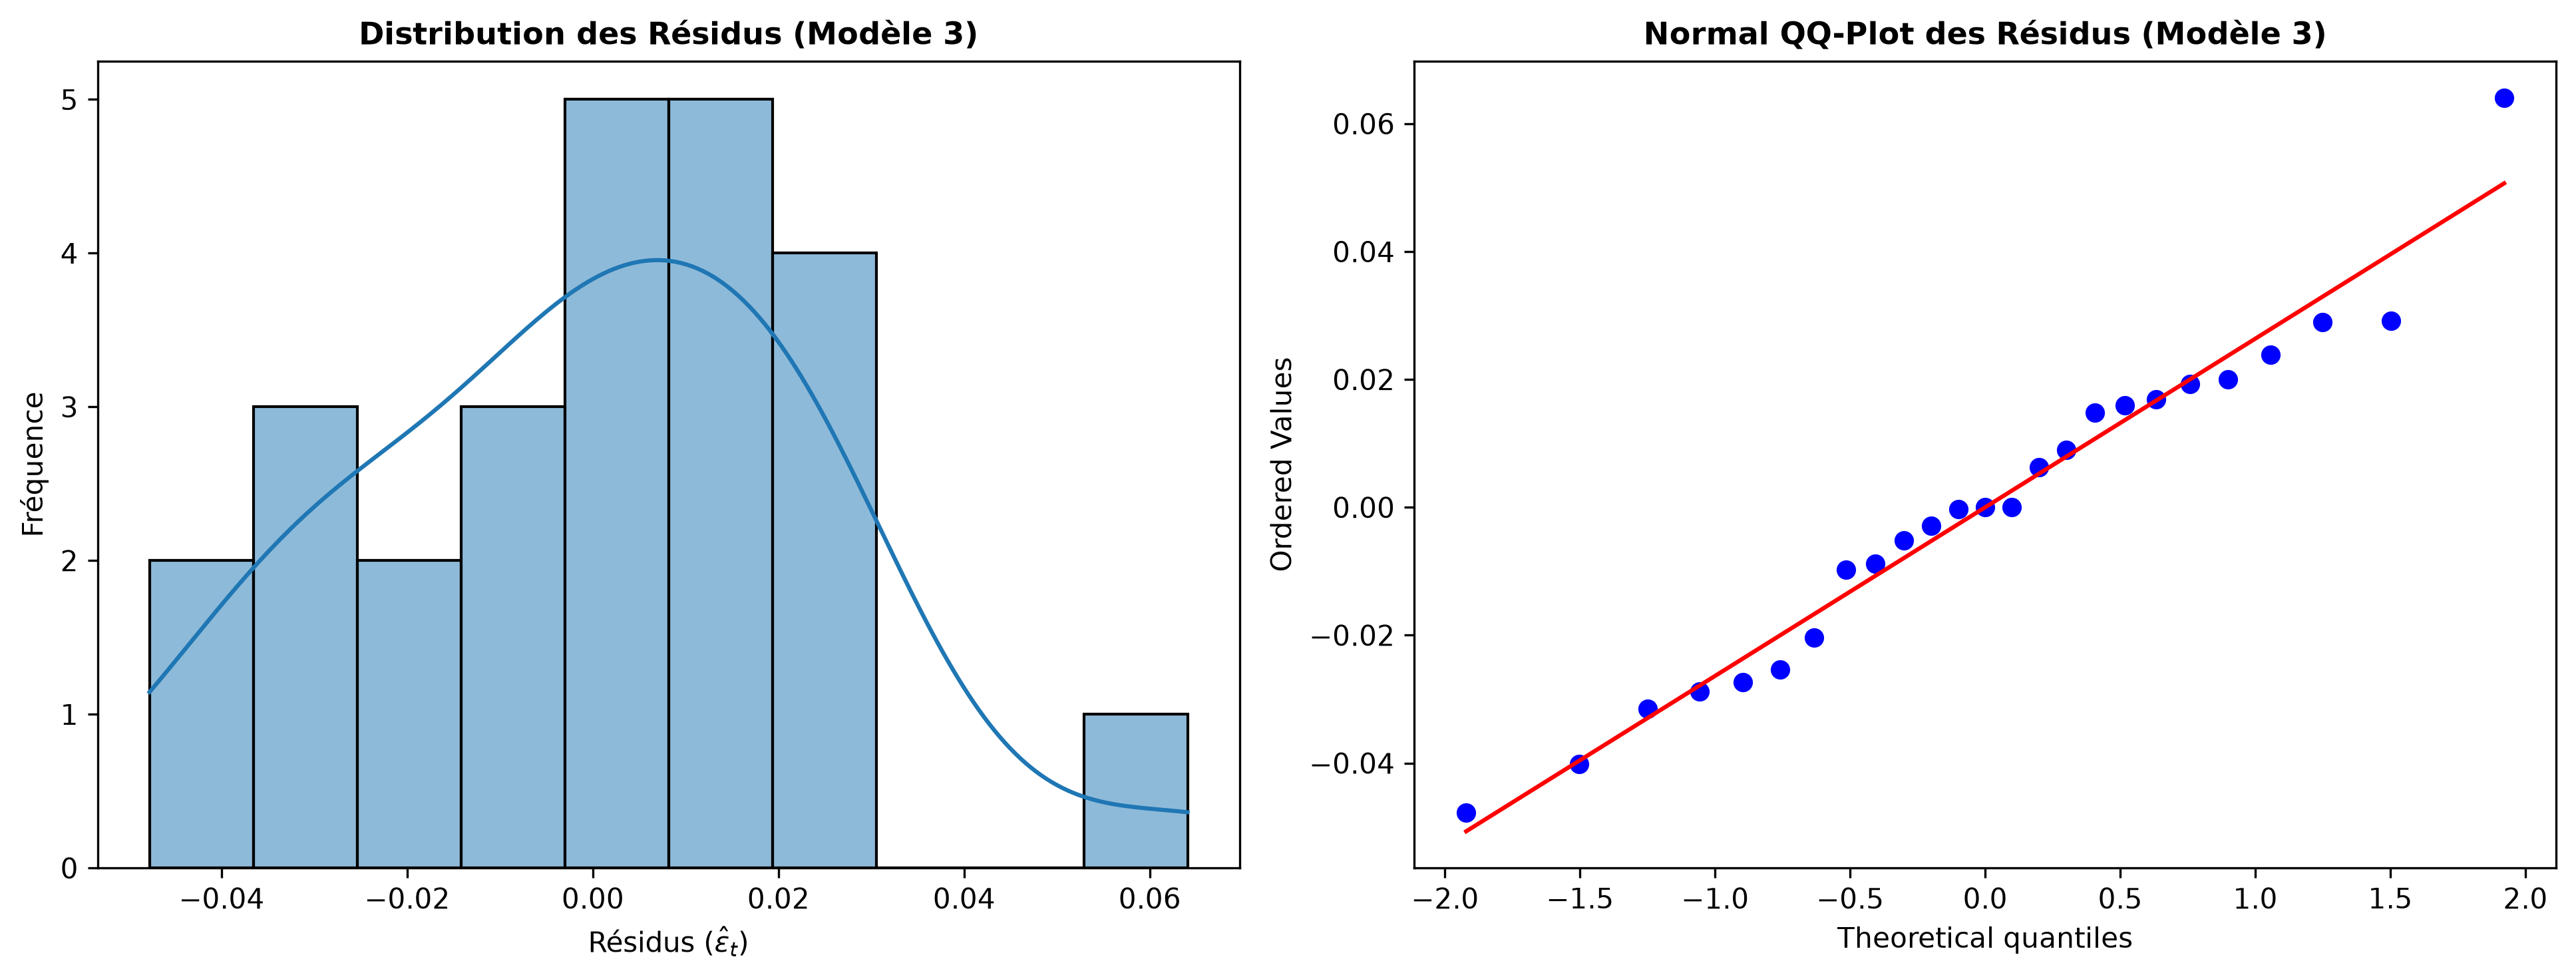
\includegraphics[width=0.88\textwidth]{outputs/figures/08_residuals_normality_qqplot.png}%
  }{%
    \rule{10cm}{5cm}%
  }
  \caption{Histogramme de distribution et Normal QQ-Plot des résidus du Modèle M3}
  \label{fig:annex_qqplot}
\end{figure}

% ==============================================================================
% BIBLIOGRAPHIE
% ==============================================================================
\newpage
\bibliographystyle{plainnat}
\bibliography{\jobname}

\end{document}